\documentclass[twoside]{book}

% Packages required by doxygen
\usepackage{calc}
\usepackage{doxygen}
\usepackage{graphicx}
\usepackage[utf8]{inputenc}
\usepackage{makeidx}
\usepackage{multicol}
\usepackage{multirow}
\usepackage{textcomp}
\usepackage[table]{xcolor}

% Font selection
\usepackage[T1]{fontenc}
\usepackage{mathptmx}
\usepackage[scaled=.90]{helvet}
\usepackage{courier}
\usepackage{amssymb}
\usepackage{sectsty}
\renewcommand{\familydefault}{\sfdefault}
\allsectionsfont{%
  \fontseries{bc}\selectfont%
  \color{darkgray}%
}
\renewcommand{\DoxyLabelFont}{%
  \fontseries{bc}\selectfont%
  \color{darkgray}%
}

% Page & text layout
\usepackage{geometry}
\geometry{%
  a4paper,%
  top=2.5cm,%
  bottom=2.5cm,%
  left=2.5cm,%
  right=2.5cm%
}
\tolerance=750
\hfuzz=15pt
\hbadness=750
\setlength{\emergencystretch}{15pt}
\setlength{\parindent}{0cm}
\setlength{\parskip}{0.2cm}
\makeatletter
\renewcommand{\paragraph}{%
  \@startsection{paragraph}{4}{0ex}{-1.0ex}{1.0ex}{%
    \normalfont\normalsize\bfseries\SS@parafont%
  }%
}
\renewcommand{\subparagraph}{%
  \@startsection{subparagraph}{5}{0ex}{-1.0ex}{1.0ex}{%
    \normalfont\normalsize\bfseries\SS@subparafont%
  }%
}
\makeatother

% Headers & footers
\usepackage{fancyhdr}
\pagestyle{fancyplain}
\fancyhead[LE]{\fancyplain{}{\bfseries\thepage}}
\fancyhead[CE]{\fancyplain{}{}}
\fancyhead[RE]{\fancyplain{}{\bfseries\leftmark}}
\fancyhead[LO]{\fancyplain{}{\bfseries\rightmark}}
\fancyhead[CO]{\fancyplain{}{}}
\fancyhead[RO]{\fancyplain{}{\bfseries\thepage}}
\fancyfoot[LE]{\fancyplain{}{}}
\fancyfoot[CE]{\fancyplain{}{}}
\fancyfoot[RE]{\fancyplain{}{\bfseries\scriptsize Generated on Mon Jul 24 2017 14\-:06\-:11 for G4\-E\-M\-M\-A Source Files by Doxygen }}
\fancyfoot[LO]{\fancyplain{}{\bfseries\scriptsize Generated on Mon Jul 24 2017 14\-:06\-:11 for G4\-E\-M\-M\-A Source Files by Doxygen }}
\fancyfoot[CO]{\fancyplain{}{}}
\fancyfoot[RO]{\fancyplain{}{}}
\renewcommand{\footrulewidth}{0.4pt}
\renewcommand{\chaptermark}[1]{%
  \markboth{#1}{}%
}
\renewcommand{\sectionmark}[1]{%
  \markright{\thesection\ #1}%
}

% Indices & bibliography
\usepackage{natbib}
\usepackage[titles]{tocloft}
\setcounter{tocdepth}{3}
\setcounter{secnumdepth}{5}
\makeindex

% Hyperlinks (required, but should be loaded last)
\usepackage{ifpdf}
\ifpdf
  \usepackage[pdftex,pagebackref=true]{hyperref}
\else
  \usepackage[ps2pdf,pagebackref=true]{hyperref}
\fi
\hypersetup{%
  colorlinks=true,%
  linkcolor=blue,%
  citecolor=blue,%
  unicode%
}

% Custom commands
\newcommand{\clearemptydoublepage}{%
  \newpage{\pagestyle{empty}\cleardoublepage}%
}


%===== C O N T E N T S =====

\begin{document}

% Titlepage & ToC
\hypersetup{pageanchor=false}
\pagenumbering{roman}
\begin{titlepage}
\vspace*{7cm}
\begin{center}%
{\Large G4\-E\-M\-M\-A Source Files }\\
\vspace*{1cm}
{\large Generated by Doxygen 1.8.6}\\
\vspace*{0.5cm}
{\small Mon Jul 24 2017 14:06:11}\\
\end{center}
\end{titlepage}
\clearemptydoublepage
\tableofcontents
\clearemptydoublepage
\pagenumbering{arabic}
\hypersetup{pageanchor=true}

%--- Begin generated contents ---
\chapter{File Index}
\section{File List}
Here is a list of all documented files with brief descriptions\-:\begin{DoxyCompactList}
\item\contentsline{section}{\hyperlink{BGField1_8hh}{B\-G\-Field1.\-hh} \\*B\-G\-Field1-\/7 are 7 almost identical headers that define 7 similar classes derived from \char`\"{}\-E\-M\-M\-A\-Element\-Field.\-hh.\char`\"{} They each descibe an E\-M field that is part of E\-M\-M\-A }{\pageref{BGField1_8hh}}{}
\item\contentsline{section}{\hyperlink{BGField2_8hh}{B\-G\-Field2.\-hh} \\*B\-G\-Field1-\/7 are 7 almost identical headers that define 7 similar classes derived from \char`\"{}\-E\-M\-M\-A\-Element\-Field.\-hh.\char`\"{} They each descibe an E\-M field that is part of E\-M\-M\-A }{\pageref{BGField2_8hh}}{}
\item\contentsline{section}{\hyperlink{BGField3_8hh}{B\-G\-Field3.\-hh} \\*B\-G\-Field1-\/7 are 7 almost identical headers that define 7 similar classes derived from \char`\"{}\-E\-M\-M\-A\-Element\-Field.\-hh.\char`\"{} They each descibe an E\-M field that is part of E\-M\-M\-A }{\pageref{BGField3_8hh}}{}
\item\contentsline{section}{\hyperlink{BGField4_8hh}{B\-G\-Field4.\-hh} \\*B\-G\-Field1-\/7 are 7 almost identical headers that define 7 similar classes derived from \char`\"{}\-E\-M\-M\-A\-Element\-Field.\-hh.\char`\"{} They each descibe an E\-M field that is part of E\-M\-M\-A }{\pageref{BGField4_8hh}}{}
\item\contentsline{section}{\hyperlink{BGField5_8hh}{B\-G\-Field5.\-hh} \\*B\-G\-Field1-\/7 are 7 almost identical headers that define 7 similar classes derived from \char`\"{}\-E\-M\-M\-A\-Element\-Field.\-hh.\char`\"{} They each descibe an E\-M field that is part of E\-M\-M\-A }{\pageref{BGField5_8hh}}{}
\item\contentsline{section}{\hyperlink{BGField6_8hh}{B\-G\-Field6.\-hh} \\*B\-G\-Field1-\/7 are 7 almost identical headers that define 7 similar classes derived from \char`\"{}\-E\-M\-M\-A\-Element\-Field.\-hh.\char`\"{} They each descibe an E\-M field that is part of E\-M\-M\-A }{\pageref{BGField6_8hh}}{}
\item\contentsline{section}{\hyperlink{BGField7_8hh}{B\-G\-Field7.\-hh} \\*B\-G\-Field1-\/7 are 7 almost identical headers that define 7 similar classes derived from \char`\"{}\-E\-M\-M\-A\-Element\-Field.\-hh.\char`\"{} They each descibe an E\-M field that is part of E\-M\-M\-A }{\pageref{BGField7_8hh}}{}
\item\contentsline{section}{\hyperlink{c2__factory_8hh}{c2\-\_\-factory.\-hh} \\*Provides a factory class to avoid an infinite number of template declarations }{\pageref{c2__factory_8hh}}{}
\item\contentsline{section}{\hyperlink{c2__function_8hh}{c2\-\_\-function.\-hh} \\*Provides the headers for the general \hyperlink{classc2__function}{c2\-\_\-function} algebra which supports fast, flexible operations on piecewise-\/twice-\/differentiable functions }{\pageref{c2__function_8hh}}{}
\item\contentsline{section}{\hyperlink{CathodeWireParameterisation_8hh}{Cathode\-Wire\-Parameterisation.\-hh} \\*This is a parameterisation that describes a series of cylinders (wires) along X }{\pageref{CathodeWireParameterisation_8hh}}{}
\item\contentsline{section}{\hyperlink{EMFieldDebugger_8hh}{E\-M\-Field\-Debugger.\-hh} \\*This header declares a class used in the corresponding source file that calculates the value of E\-M fields at different locations in the simulation }{\pageref{EMFieldDebugger_8hh}}{}
\item\contentsline{section}{\hyperlink{EMMAAnalysisManager_8hh}{E\-M\-M\-A\-Analysis\-Manager.\-hh} \\*This header calls upon several root files and declares other functions for a source file. These functions call upon and write to R\-O\-O\-T files to display simulation outcomes or results }{\pageref{EMMAAnalysisManager_8hh}}{}
\item\contentsline{section}{\hyperlink{EMMADetectorConstMessenger_8hh}{E\-M\-M\-A\-Detector\-Const\-Messenger.\-hh} \\*This header file contains deals with user commands relating to detector construction }{\pageref{EMMADetectorConstMessenger_8hh}}{}
\item\contentsline{section}{\hyperlink{EMMADetectorConstruction_8hh}{E\-M\-M\-A\-Detector\-Construction.\-hh} \\*This header file builds on the G4 header \char`\"{}\-G4\-V\-User\-Detector\-Construction.\-hh\char`\"{} to set the global G4 variables specifying the materials and simulation attributes of the E\-M\-M\-A detectors. Several E\-M\-M\-A functions (regarding its detectors) are also defined }{\pageref{EMMADetectorConstruction_8hh}}{}
\item\contentsline{section}{\hyperlink{EMMADriftChamber_8hh}{E\-M\-M\-A\-Drift\-Chamber.\-hh} \\*This header contains the class required to run the P\-G\-A\-C drift chamber (see also G4\-Sensitive\-Detector.\-hh) }{\pageref{EMMADriftChamber_8hh}}{}
\item\contentsline{section}{\hyperlink{EMMADriftChamberHit_8hh}{E\-M\-M\-A\-Drift\-Chamber\-Hit.\-hh} \\*This class manages the hit object in regards to the drift chamber part of the simulation. It defines global variables and functions for the G4 code to run necessary hit simulations. The virtual methods draw() and print() are used. For further details about each part of this file, examine the accompanying explanations adjacent to the classes }{\pageref{EMMADriftChamberHit_8hh}}{}
\item\contentsline{section}{\hyperlink{EMMAElementField_8hh}{E\-M\-M\-A\-Element\-Field.\-hh} \\*This is the interface class used by Global\-Field to compute the field value at a given point\mbox{[}\mbox{]} }{\pageref{EMMAElementField_8hh}}{}
\item\contentsline{section}{\hyperlink{EMMAEMPhysics_8hh}{E\-M\-M\-A\-E\-M\-Physics.\-hh} \\*The G4 header \char`\"{}\-G4\-V\-Physics\-Constructor.\-hh\char`\"{} contains a virtual class that must be used to create concrete classes for specific applications (such as E\-M\-M\-A). This header builds such a concrete class to include E\-M\-M\-A's specific particles and processes. Specifically, this header defines particles and processes required to simulate E\-M interactions }{\pageref{EMMAEMPhysics_8hh}}{}
\item\contentsline{section}{\hyperlink{EMMAEventAction_8hh}{E\-M\-M\-A\-Event\-Action.\-hh} \\*This header defines the user's action class, and specifically, the beginning and end of a user action. It generates from the Primary\-Generator headers as the user begins an action. Contains functions that are invoked by G4\-Event\-Manager }{\pageref{EMMAEventAction_8hh}}{}
\item\contentsline{section}{\hyperlink{EMMAEventActionMessenger_8hh}{E\-M\-M\-A\-Event\-Action\-Messenger.\-hh} \\*This file is responsible for deleting commands, delivering commands to destination classes, defining global G4 variables specific to E\-M\-M\-A, and replying the current values of the parameters (again as described the \char`\"{}\-G4\-U\-Imessenger.\-hh\char`\"{} source file) regarding the event action (from the primary generator) }{\pageref{EMMAEventActionMessenger_8hh}}{}
\item\contentsline{section}{\hyperlink{EMMAGeneralPhysics_8hh}{E\-M\-M\-A\-General\-Physics.\-hh} \\*This header defines particles and processes required for other more specific physics processes }{\pageref{EMMAGeneralPhysics_8hh}}{}
\item\contentsline{section}{\hyperlink{EMMAGlobalField_8hh}{E\-M\-M\-A\-Global\-Field.\-hh} \\*Handles the global Electro\-Magnetic field }{\pageref{EMMAGlobalField_8hh}}{}
\item\contentsline{section}{\hyperlink{EMMAHadronPhysics_8hh}{E\-M\-M\-A\-Hadron\-Physics.\-hh} \\*The G4 header \char`\"{}\-G4\-V\-Physics\-Constructor.\-hh\char`\"{} contains a virtual class that must be used to create concrete classes for specific applications (such as E\-M\-M\-A). Specifically, this header defines particles and processes required to simulate hadron interactions }{\pageref{EMMAHadronPhysics_8hh}}{}
\item\contentsline{section}{\hyperlink{EMMAIonChamber_8hh}{E\-M\-M\-A\-Ion\-Chamber.\-hh} \\*This defines a calorimeter sensitive detector class (ion chamber). Uses the inherited G4 detector construction classes to build the operation of the ion chamber }{\pageref{EMMAIonChamber_8hh}}{}
\item\contentsline{section}{\hyperlink{EMMAIonChamberHit_8hh}{E\-M\-M\-A\-Ion\-Chamber\-Hit.\-hh} \\*Calorimeter (ion chamber) hit class\-: defines data members to store the the energy deposit and track lengths of charged particles in a selected volume }{\pageref{EMMAIonChamberHit_8hh}}{}
\item\contentsline{section}{\hyperlink{EMMAIonPhysics_8hh}{E\-M\-M\-A\-Ion\-Physics.\-hh} \\*The G4 header \char`\"{}\-G4\-V\-Physics\-Constructor.\-hh\char`\"{} contains a virtual class that must be used to create concrete classes for specific applications (such as E\-M\-M\-A). Specifically, this header defines particles and processes required to simulate ion interactions }{\pageref{EMMAIonPhysics_8hh}}{}
\item\contentsline{section}{\hyperlink{EMMAIonPhysicsMessenger_8hh}{E\-M\-M\-A\-Ion\-Physics\-Messenger.\-hh} \\*This header file contains deals with user commands relating to ionic physics processes }{\pageref{EMMAIonPhysicsMessenger_8hh}}{}
\item\contentsline{section}{\hyperlink{EMMAMuonPhysics_8hh}{E\-M\-M\-A\-Muon\-Physics.\-hh} \\*The G4 header \char`\"{}\-G4\-V\-Physics\-Constructor.\-hh\char`\"{} contains a virtual class that must be used to create concrete classes for specific applications (such as E\-M\-M\-A). Specifically, this header defines particles and processes required to simulate muon interactions }{\pageref{EMMAMuonPhysics_8hh}}{}
\item\contentsline{section}{\hyperlink{EMMANuclearReactionDataSet_8hh}{E\-M\-M\-A\-Nuclear\-Reaction\-Data\-Set.\-hh} \\*Data set for (two body) nuclear reaction cross sections. Inherited from similar G4 headers }{\pageref{EMMANuclearReactionDataSet_8hh}}{}
\item\contentsline{section}{\hyperlink{EMMANuclearReactionProcess_8hh}{E\-M\-M\-A\-Nuclear\-Reaction\-Process.\-hh} \\*Nuclear-\/reaction process for projectile (Z1,A1) striking target (Z2,A2) with cross section (cs) }{\pageref{EMMANuclearReactionProcess_8hh}}{}
\item\contentsline{section}{\hyperlink{EMMANuclearReactionTwoBody_8hh}{E\-M\-M\-A\-Nuclear\-Reaction\-Two\-Body.\-hh} \\*Nuclear-\/reaction model for two-\/body final-\/state (Z3,A3)+(Z4,A4) after a two body reaction between a projectile and target }{\pageref{EMMANuclearReactionTwoBody_8hh}}{}
\item\contentsline{section}{\hyperlink{EMMAPhysicsList_8hh}{E\-M\-M\-A\-Physics\-List.\-hh} \\*E\-M\-M\-A's specific objects and particles are registered from the virtual class in \char`\"{}\-G4\-V\-Physics\-Constructor.\-hh.\char`\"{} These objects are registered to G4\-User\-Physics\-List, which is the parent of \char`\"{}\-G4\-V\-Modular\-Physics\-List.\-hh.\char`\"{} This header defines a concrete class inherited from \char`\"{}\-G4\-V\-Modular\-Physics\-List.\-hh\char`\"{} }{\pageref{EMMAPhysicsList_8hh}}{}
\item\contentsline{section}{\hyperlink{EMMAPrimaryGeneratorAction_8hh}{E\-M\-M\-A\-Primary\-Generator\-Action.\-hh} \\*This is an important class responsible for primary particle or vertex generation. It is required by G4; the Primary Generator is not an actual physical component of E\-M\-M\-A but rather a G4 construction element. This class is the concrete class stemming from the virtual class found in \char`\"{}\-G4\-V\-User\-Primary\-Generator\-Action.\-hh.\char`\"{} }{\pageref{EMMAPrimaryGeneratorAction_8hh}}{}
\item\contentsline{section}{\hyperlink{EMMAPrimaryGeneratorMessenger_8hh}{E\-M\-M\-A\-Primary\-Generator\-Messenger.\-hh} \\*This file is responsible for deleting commands, delivering commands to destination classes, defining global G4 variables specific to E\-M\-M\-A, and replying the current values of the parameters (again as described the \char`\"{}\-G4\-U\-Imessenger.\-hh\char`\"{} source file) regarding the primary generator (of the events) }{\pageref{EMMAPrimaryGeneratorMessenger_8hh}}{}
\item\contentsline{section}{\hyperlink{EMMASteppingAction_8hh}{E\-M\-M\-A\-Stepping\-Action.\-hh} \\*Headers that have to do with \char`\"{}stepping\char`\"{} (loops) is related to tracking the particle and its interactions with its surroundings. This class defines functions that build on \char`\"{}\-G4\-User\-Stepping\-Action.\-hh,\char`\"{} which represents user actions during \char`\"{}stepping.\char`\"{} }{\pageref{EMMASteppingAction_8hh}}{}
\item\contentsline{section}{\hyperlink{EMMASteppingVerbose_8hh}{E\-M\-M\-A\-Stepping\-Verbose.\-hh} \\*This class manages the verbose outputs in G4\-Stepping\-Manager. It shows how to extract information during the tracking of a particle }{\pageref{EMMASteppingVerbose_8hh}}{}
\item\contentsline{section}{\hyperlink{F04StepMax_8hh}{F04\-Step\-Max.\-hh} \\*Header defines a class relating to the step (tracking) of a particle involved in a discrete process. For more general information see this header's dependencies }{\pageref{F04StepMax_8hh}}{}
\item\contentsline{section}{\hyperlink{G4LindhardPartition_8hh}{G4\-Lindhard\-Partition.\-hh} \\*A seemingly periphery code that calculates the non-\/ionizing energy loss of radiation via the Lindhard partition function. Used to calculate energy deposited in target by the beam thereby affecting energy of recoils }{\pageref{G4LindhardPartition_8hh}}{}
\item\contentsline{section}{\hyperlink{G4ScreenedNuclearRecoil_8hh}{G4\-Screened\-Nuclear\-Recoil.\-hh} \\*Builds the process of screened electromagnetic nuclear elastic scattering. Declares many functions primarily used for coulomb interactions between nuclei }{\pageref{G4ScreenedNuclearRecoil_8hh}}{}
\item\contentsline{section}{\hyperlink{PGACWireParameterisation_8hh}{P\-G\-A\-C\-Wire\-Parameterisation.\-hh} \\*A parameterisation that describes a series of cylinders along Z (the wires in the P\-C\-A\-G ioin drift chamber) }{\pageref{PGACWireParameterisation_8hh}}{}
\item\contentsline{section}{\hyperlink{SpectrometerConstruction_8hh}{Spectrometer\-Construction.\-hh} \\*Builds the E\-M\-M\-A spectrometer through defining classes and variables, including those for slit control. This header is built upon the virtual classes inherited from \char`\"{}\-G4\-V\-User\-Detector\-Construction.\-hh.\char`\"{} }{\pageref{SpectrometerConstruction_8hh}}{}
\item\contentsline{section}{{\bfseries Stacking\-Action.\-hh} }{\pageref{StackingAction_8hh}}{}
\item\contentsline{section}{{\bfseries Tracking\-Action.\-hh} }{\pageref{TrackingAction_8hh}}{}
\end{DoxyCompactList}

\chapter{File Documentation}
\hypertarget{BGField1_8cc}{\section{B\-G\-Field1.\-cc File Reference}
\label{BGField1_8cc}\index{B\-G\-Field1.\-cc@{B\-G\-Field1.\-cc}}
}


The B\-G\-Field source files construct the 7 magnetic and electric fields on the E\-M\-M\-A simulation (Q\-Q\-E\-M\-E\-Q\-Q).  


{\ttfamily \#include \char`\"{}B\-G\-Field1.\-hh\char`\"{}}\\*
{\ttfamily \#include \char`\"{}fortran\-\_\-subs.\-inc\char`\"{}}\\*
{\ttfamily \#include \char`\"{}G4ios.\-hh\char`\"{}}\\*
{\ttfamily \#include \char`\"{}G4\-Units\-Table.\-hh\char`\"{}}\\*
{\ttfamily \#include $<$fstream$>$}\\*
{\ttfamily \#include \char`\"{}E\-M\-M\-A\-Element\-Field.\-hh\char`\"{}}\\*


\subsection{Detailed Description}
The B\-G\-Field source files construct the 7 magnetic and electric fields on the E\-M\-M\-A simulation (Q\-Q\-E\-M\-E\-Q\-Q). 
\hypertarget{BGField2_8cc}{}\section{B\+G\+Field2.\+cc File Reference}
\label{BGField2_8cc}\index{B\+G\+Field2.\+cc@{B\+G\+Field2.\+cc}}
{\ttfamily \#include \char`\"{}B\+G\+Field2.\+hh\char`\"{}}\\*
{\ttfamily \#include \char`\"{}fortran\+\_\+subs.\+inc\char`\"{}}\\*
{\ttfamily \#include \char`\"{}G4\+Units\+Table.\+hh\char`\"{}}\\*
{\ttfamily \#include $<$fstream$>$}\\*
{\ttfamily \#include \char`\"{}E\+M\+M\+A\+Global\+Field.\+hh\char`\"{}}\\*
Include dependency graph for B\+G\+Field2.\+cc\+:
\nopagebreak
\begin{figure}[H]
\begin{center}
\leavevmode
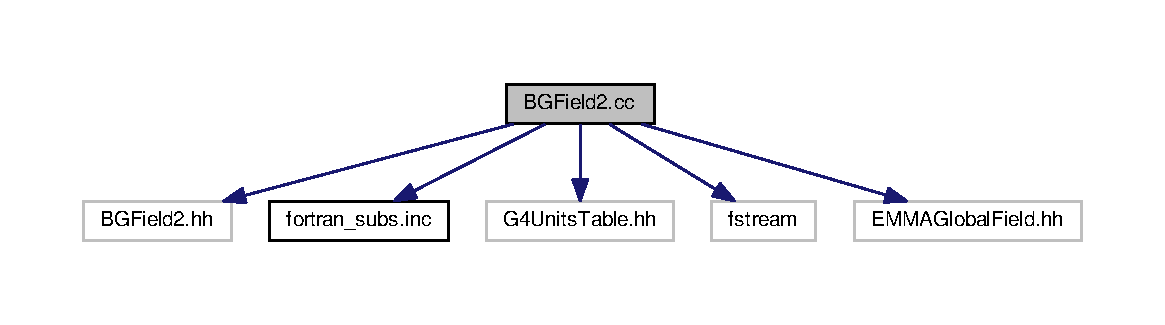
\includegraphics[width=350pt]{BGField2_8cc__incl}
\end{center}
\end{figure}

\hypertarget{BGField3_8cc}{}\section{B\+G\+Field3.\+cc File Reference}
\label{BGField3_8cc}\index{B\+G\+Field3.\+cc@{B\+G\+Field3.\+cc}}
{\ttfamily \#include \char`\"{}B\+G\+Field3.\+hh\char`\"{}}\\*
{\ttfamily \#include \char`\"{}fortran\+\_\+subs.\+inc\char`\"{}}\\*
{\ttfamily \#include \char`\"{}G4\+Units\+Table.\+hh\char`\"{}}\\*
{\ttfamily \#include $<$fstream$>$}\\*
{\ttfamily \#include \char`\"{}E\+M\+M\+A\+Global\+Field.\+hh\char`\"{}}\\*
Include dependency graph for B\+G\+Field3.\+cc\+:
\nopagebreak
\begin{figure}[H]
\begin{center}
\leavevmode
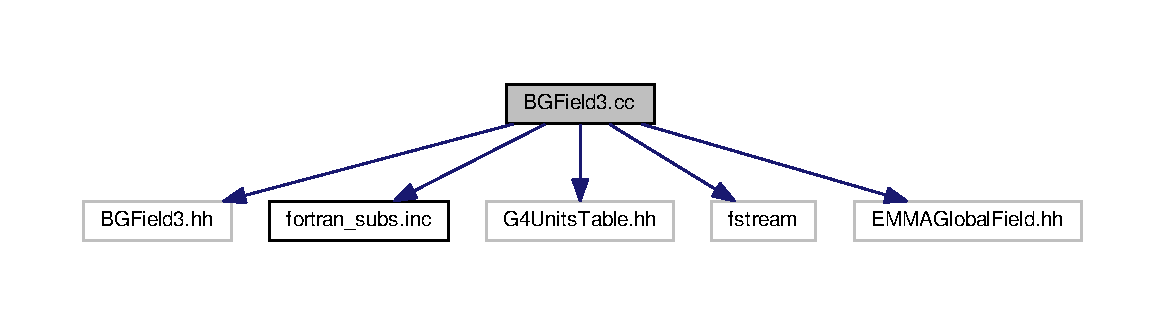
\includegraphics[width=350pt]{BGField3_8cc__incl}
\end{center}
\end{figure}

\hypertarget{BGField4_8cc}{\section{B\-G\-Field4.\-cc File Reference}
\label{BGField4_8cc}\index{B\-G\-Field4.\-cc@{B\-G\-Field4.\-cc}}
}


The B\-G\-Field source files construct the 7 magnetic and electric fields on the E\-M\-M\-A simulation (Q\-Q\-E\-M\-E\-Q\-Q).  


{\ttfamily \#include \char`\"{}B\-G\-Field4.\-hh\char`\"{}}\\*
{\ttfamily \#include \char`\"{}fortran\-\_\-subs.\-inc\char`\"{}}\\*
{\ttfamily \#include \char`\"{}G4\-Units\-Table.\-hh\char`\"{}}\\*
{\ttfamily \#include \char`\"{}E\-M\-M\-A\-Global\-Field.\-hh\char`\"{}}\\*
{\ttfamily \#include $<$fstream$>$}\\*


\subsection{Detailed Description}
The B\-G\-Field source files construct the 7 magnetic and electric fields on the E\-M\-M\-A simulation (Q\-Q\-E\-M\-E\-Q\-Q). 
\hypertarget{BGField5_8cc}{\section{B\-G\-Field5.\-cc File Reference}
\label{BGField5_8cc}\index{B\-G\-Field5.\-cc@{B\-G\-Field5.\-cc}}
}


The B\-G\-Field source files construct the 7 magnetic and electric fields on the E\-M\-M\-A simulation (Q\-Q\-E\-M\-E\-Q\-Q).  


{\ttfamily \#include \char`\"{}B\-G\-Field5.\-hh\char`\"{}}\\*
{\ttfamily \#include \char`\"{}fortran\-\_\-subs.\-inc\char`\"{}}\\*
{\ttfamily \#include \char`\"{}G4\-Units\-Table.\-hh\char`\"{}}\\*
{\ttfamily \#include $<$fstream$>$}\\*
{\ttfamily \#include \char`\"{}E\-M\-M\-A\-Global\-Field.\-hh\char`\"{}}\\*


\subsection{Detailed Description}
The B\-G\-Field source files construct the 7 magnetic and electric fields on the E\-M\-M\-A simulation (Q\-Q\-E\-M\-E\-Q\-Q). 
\hypertarget{BGField6_8cc}{}\section{B\+G\+Field6.\+cc File Reference}
\label{BGField6_8cc}\index{B\+G\+Field6.\+cc@{B\+G\+Field6.\+cc}}
{\ttfamily \#include \char`\"{}B\+G\+Field6.\+hh\char`\"{}}\\*
{\ttfamily \#include \char`\"{}fortran\+\_\+subs.\+inc\char`\"{}}\\*
{\ttfamily \#include \char`\"{}G4\+Units\+Table.\+hh\char`\"{}}\\*
{\ttfamily \#include $<$fstream$>$}\\*
{\ttfamily \#include \char`\"{}E\+M\+M\+A\+Global\+Field.\+hh\char`\"{}}\\*
Include dependency graph for B\+G\+Field6.\+cc\+:
\nopagebreak
\begin{figure}[H]
\begin{center}
\leavevmode
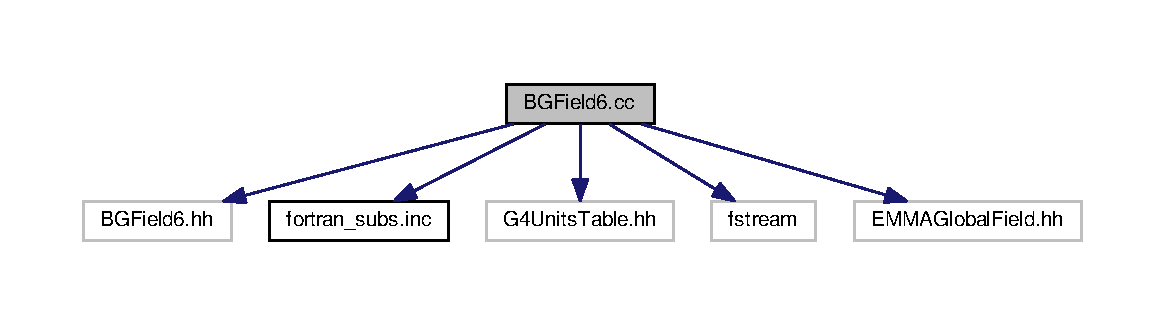
\includegraphics[width=350pt]{BGField6_8cc__incl}
\end{center}
\end{figure}

\hypertarget{BGField7_8cc}{}\section{B\+G\+Field7.\+cc File Reference}
\label{BGField7_8cc}\index{B\+G\+Field7.\+cc@{B\+G\+Field7.\+cc}}
{\ttfamily \#include \char`\"{}B\+G\+Field7.\+hh\char`\"{}}\\*
{\ttfamily \#include \char`\"{}fortran\+\_\+subs.\+inc\char`\"{}}\\*
{\ttfamily \#include \char`\"{}G4\+Units\+Table.\+hh\char`\"{}}\\*
{\ttfamily \#include $<$fstream$>$}\\*
{\ttfamily \#include \char`\"{}E\+M\+M\+A\+Global\+Field.\+hh\char`\"{}}\\*
Include dependency graph for B\+G\+Field7.\+cc\+:
\nopagebreak
\begin{figure}[H]
\begin{center}
\leavevmode
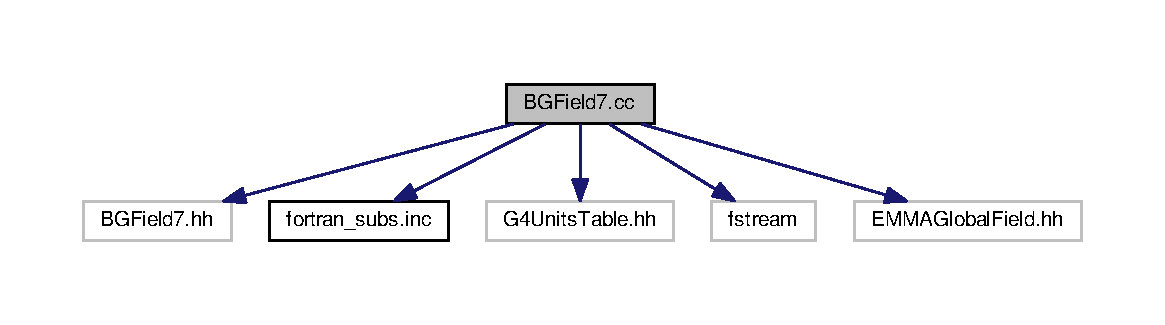
\includegraphics[width=350pt]{BGField7_8cc__incl}
\end{center}
\end{figure}

\hypertarget{EMFieldDebugger_8cc}{}\section{E\+M\+Field\+Debugger.\+cc File Reference}
\label{EMFieldDebugger_8cc}\index{E\+M\+Field\+Debugger.\+cc@{E\+M\+Field\+Debugger.\+cc}}
{\ttfamily \#include \char`\"{}E\+M\+Field\+Debugger.\+hh\char`\"{}}\\*
{\ttfamily \#include \char`\"{}E\+M\+M\+A\+Global\+Field.\+hh\char`\"{}}\\*
{\ttfamily \#include \char`\"{}G4\+Units\+Table.\+hh\char`\"{}}\\*
{\ttfamily \#include $<$iomanip$>$}\\*
{\ttfamily \#include $<$fstream$>$}\\*
{\ttfamily \#include $<$stdlib.\+h$>$}\\*
{\ttfamily \#include \char`\"{}G4\+System\+Of\+Units.\+hh\char`\"{}}\\*
Include dependency graph for E\+M\+Field\+Debugger.\+cc\+:
\nopagebreak
\begin{figure}[H]
\begin{center}
\leavevmode
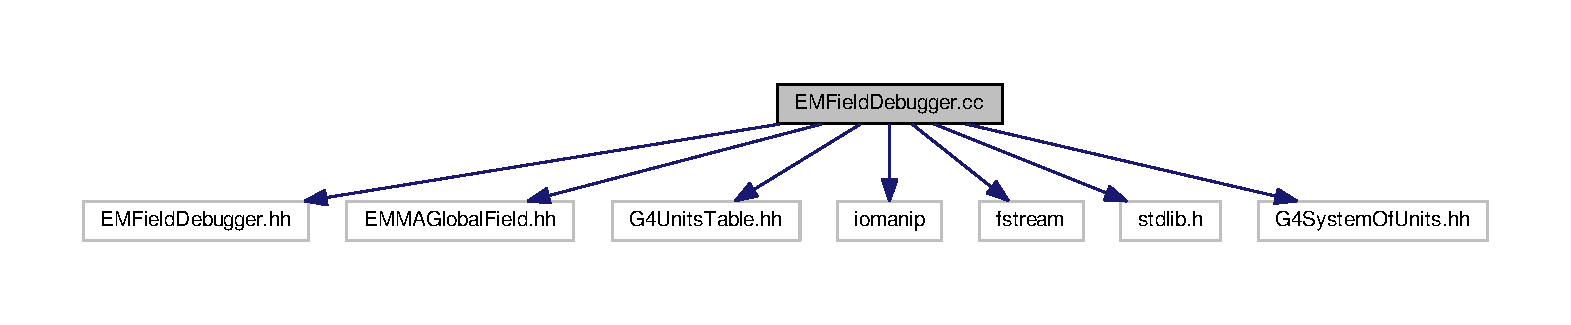
\includegraphics[width=350pt]{EMFieldDebugger_8cc__incl}
\end{center}
\end{figure}

\hypertarget{EMMAAnalysisManager_8cc}{\section{E\-M\-M\-A\-Analysis\-Manager.\-cc File Reference}
\label{EMMAAnalysisManager_8cc}\index{E\-M\-M\-A\-Analysis\-Manager.\-cc@{E\-M\-M\-A\-Analysis\-Manager.\-cc}}
}


Calls upon and writes to R\-O\-O\-T files to display results and outcomes.  




\subsection{Detailed Description}
Calls upon and writes to R\-O\-O\-T files to display results and outcomes. 
\hypertarget{EMMADetectorConstMessenger_8cc}{\section{E\-M\-M\-A\-Detector\-Const\-Messenger.\-cc File Reference}
\label{EMMADetectorConstMessenger_8cc}\index{E\-M\-M\-A\-Detector\-Const\-Messenger.\-cc@{E\-M\-M\-A\-Detector\-Const\-Messenger.\-cc}}
}


Connects U\-I and user input to the detector construction. Takes and gives use commands to/from the user when constructing detectors (the P\-G\-A\-C, the degraders, etc.).  


{\ttfamily \#include \char`\"{}E\-M\-M\-A\-Detector\-Const\-Messenger.\-hh\char`\"{}}\\*
{\ttfamily \#include \char`\"{}E\-M\-M\-A\-Detector\-Construction.\-hh\char`\"{}}\\*
{\ttfamily \#include \char`\"{}G4\-U\-Idirectory.\-hh\char`\"{}}\\*
{\ttfamily \#include \char`\"{}G4\-U\-Icmd\-With\-A\-Double\-And\-Unit.\-hh\char`\"{}}\\*
{\ttfamily \#include \char`\"{}G4\-U\-Icmd\-With\-A\-Double.\-hh\char`\"{}}\\*
{\ttfamily \#include \char`\"{}G4\-U\-Icmd\-Without\-Parameter.\-hh\char`\"{}}\\*
{\ttfamily \#include \char`\"{}G4ios.\-hh\char`\"{}}\\*


\subsection{Detailed Description}
Connects U\-I and user input to the detector construction. Takes and gives use commands to/from the user when constructing detectors (the P\-G\-A\-C, the degraders, etc.). 
\hypertarget{EMMADetectorConstruction_8cc}{}\section{E\+M\+M\+A\+Detector\+Construction.\+cc File Reference}
\label{EMMADetectorConstruction_8cc}\index{E\+M\+M\+A\+Detector\+Construction.\+cc@{E\+M\+M\+A\+Detector\+Construction.\+cc}}
{\ttfamily \#include \char`\"{}E\+M\+M\+A\+Detector\+Construction.\+hh\char`\"{}}\\*
{\ttfamily \#include \char`\"{}G4\+Field\+Manager.\+hh\char`\"{}}\\*
{\ttfamily \#include \char`\"{}G4\+Transportation\+Manager.\+hh\char`\"{}}\\*
{\ttfamily \#include \char`\"{}G4\+Mag\+\_\+\+Usual\+Eq\+Rhs.\+hh\char`\"{}}\\*
{\ttfamily \#include \char`\"{}G4\+Material.\+hh\char`\"{}}\\*
{\ttfamily \#include \char`\"{}G4\+Element.\+hh\char`\"{}}\\*
{\ttfamily \#include \char`\"{}G4\+Material\+Table.\+hh\char`\"{}}\\*
{\ttfamily \#include \char`\"{}G4\+Nist\+Manager.\+hh\char`\"{}}\\*
{\ttfamily \#include \char`\"{}G4\+V\+Solid.\+hh\char`\"{}}\\*
{\ttfamily \#include \char`\"{}G4\+Union\+Solid.\+hh\char`\"{}}\\*
{\ttfamily \#include \char`\"{}G4\+Box.\+hh\char`\"{}}\\*
{\ttfamily \#include \char`\"{}G4\+Tubs.\+hh\char`\"{}}\\*
{\ttfamily \#include \char`\"{}G4\+Logical\+Volume.\+hh\char`\"{}}\\*
{\ttfamily \#include \char`\"{}G4\+V\+Physical\+Volume.\+hh\char`\"{}}\\*
{\ttfamily \#include \char`\"{}G4\+P\+V\+Placement.\+hh\char`\"{}}\\*
{\ttfamily \#include \char`\"{}G4\+P\+V\+Replica.\+hh\char`\"{}}\\*
{\ttfamily \#include \char`\"{}G4\+P\+V\+Parameterised.\+hh\char`\"{}}\\*
{\ttfamily \#include \char`\"{}G4\+User\+Limits.\+hh\char`\"{}}\\*
{\ttfamily \#include \char`\"{}G4\+Trap.\+hh\char`\"{}}\\*
{\ttfamily \#include \char`\"{}G4\+Transform3\+D.\+hh\char`\"{}}\\*
{\ttfamily \#include \char`\"{}G4\+Region.\+hh\char`\"{}}\\*
{\ttfamily \#include \char`\"{}G4\+Region\+Store.\+hh\char`\"{}}\\*
{\ttfamily \#include \char`\"{}G4\+Units\+Table.\+hh\char`\"{}}\\*
{\ttfamily \#include \char`\"{}G4\+Subtraction\+Solid.\+hh\char`\"{}}\\*
{\ttfamily \#include \char`\"{}G4\+System\+Of\+Units.\+hh\char`\"{}}\\*
{\ttfamily \#include \char`\"{}G4\+S\+D\+Manager.\+hh\char`\"{}}\\*
{\ttfamily \#include \char`\"{}G4\+V\+Sensitive\+Detector.\+hh\char`\"{}}\\*
{\ttfamily \#include \char`\"{}G4\+Run\+Manager.\+hh\char`\"{}}\\*
{\ttfamily \#include \char`\"{}G4\+Vis\+Attributes.\+hh\char`\"{}}\\*
{\ttfamily \#include \char`\"{}G4\+Colour.\+hh\char`\"{}}\\*
{\ttfamily \#include \char`\"{}G4ios.\+hh\char`\"{}}\\*
{\ttfamily \#include \char`\"{}E\+M\+M\+A\+Detector\+Const\+Messenger.\+hh\char`\"{}}\\*
{\ttfamily \#include \char`\"{}E\+M\+M\+A\+Drift\+Chamber.\+hh\char`\"{}}\\*
{\ttfamily \#include \char`\"{}E\+M\+M\+A\+Ion\+Chamber.\+hh\char`\"{}}\\*
{\ttfamily \#include \char`\"{}Spectrometer\+Construction.\+hh\char`\"{}}\\*
{\ttfamily \#include \char`\"{}E\+M\+Field\+Debugger.\+hh\char`\"{}}\\*
{\ttfamily \#include \char`\"{}Cathode\+Wire\+Parameterisation.\+hh\char`\"{}}\\*
{\ttfamily \#include \char`\"{}C\+L\+H\+E\+P/\+Units/\+System\+Of\+Units.\+h\char`\"{}}\\*
{\ttfamily \#include \char`\"{}G4\+Uniform\+Mag\+Field.\+hh\char`\"{}}\\*
{\ttfamily \#include $<$fstream$>$}\\*
{\ttfamily \#include $<$stdlib.\+h$>$}\\*
Include dependency graph for E\+M\+M\+A\+Detector\+Construction.\+cc\+:
\nopagebreak
\begin{figure}[H]
\begin{center}
\leavevmode

\includegraphics[width=350pt]{EMMADetectorConstruction_8cc__incl}
\end{center}
\end{figure}
\subsection*{Variables}
\begin{DoxyCompactItemize}
\item 
G4double \hyperlink{EMMADetectorConstruction_8cc_aeb29decdede3d925164d390a2bf4a67a}{magnetic\+Scaling} = 1
\item 
G4double \hyperlink{EMMADetectorConstruction_8cc_a528ee0b2618db44ed7b0734789834f3d}{electric\+Scaling} = 1
\item 
G4double \hyperlink{EMMADetectorConstruction_8cc_a168924eff042d94e1e59a05bbcdcca38}{target\+Thickness}
\item 
G4double \hyperlink{EMMADetectorConstruction_8cc_a7d65bdf83ece33e0fa248e3da81e825a}{target\+Zoffset}
\end{DoxyCompactItemize}


\subsection{Variable Documentation}
\index{E\+M\+M\+A\+Detector\+Construction.\+cc@{E\+M\+M\+A\+Detector\+Construction.\+cc}!electric\+Scaling@{electric\+Scaling}}
\index{electric\+Scaling@{electric\+Scaling}!E\+M\+M\+A\+Detector\+Construction.\+cc@{E\+M\+M\+A\+Detector\+Construction.\+cc}}
\subsubsection[{\texorpdfstring{electric\+Scaling}{electricScaling}}]{\setlength{\rightskip}{0pt plus 5cm}G4double electric\+Scaling = 1}\hypertarget{EMMADetectorConstruction_8cc_a528ee0b2618db44ed7b0734789834f3d}{}\label{EMMADetectorConstruction_8cc_a528ee0b2618db44ed7b0734789834f3d}
\index{E\+M\+M\+A\+Detector\+Construction.\+cc@{E\+M\+M\+A\+Detector\+Construction.\+cc}!magnetic\+Scaling@{magnetic\+Scaling}}
\index{magnetic\+Scaling@{magnetic\+Scaling}!E\+M\+M\+A\+Detector\+Construction.\+cc@{E\+M\+M\+A\+Detector\+Construction.\+cc}}
\subsubsection[{\texorpdfstring{magnetic\+Scaling}{magneticScaling}}]{\setlength{\rightskip}{0pt plus 5cm}G4double magnetic\+Scaling = 1}\hypertarget{EMMADetectorConstruction_8cc_aeb29decdede3d925164d390a2bf4a67a}{}\label{EMMADetectorConstruction_8cc_aeb29decdede3d925164d390a2bf4a67a}
\index{E\+M\+M\+A\+Detector\+Construction.\+cc@{E\+M\+M\+A\+Detector\+Construction.\+cc}!target\+Thickness@{target\+Thickness}}
\index{target\+Thickness@{target\+Thickness}!E\+M\+M\+A\+Detector\+Construction.\+cc@{E\+M\+M\+A\+Detector\+Construction.\+cc}}
\subsubsection[{\texorpdfstring{target\+Thickness}{targetThickness}}]{\setlength{\rightskip}{0pt plus 5cm}G4double target\+Thickness}\hypertarget{EMMADetectorConstruction_8cc_a168924eff042d94e1e59a05bbcdcca38}{}\label{EMMADetectorConstruction_8cc_a168924eff042d94e1e59a05bbcdcca38}
\index{E\+M\+M\+A\+Detector\+Construction.\+cc@{E\+M\+M\+A\+Detector\+Construction.\+cc}!target\+Zoffset@{target\+Zoffset}}
\index{target\+Zoffset@{target\+Zoffset}!E\+M\+M\+A\+Detector\+Construction.\+cc@{E\+M\+M\+A\+Detector\+Construction.\+cc}}
\subsubsection[{\texorpdfstring{target\+Zoffset}{targetZoffset}}]{\setlength{\rightskip}{0pt plus 5cm}G4double target\+Zoffset}\hypertarget{EMMADetectorConstruction_8cc_a7d65bdf83ece33e0fa248e3da81e825a}{}\label{EMMADetectorConstruction_8cc_a7d65bdf83ece33e0fa248e3da81e825a}

\hypertarget{EMMADriftChamber_8cc}{\section{E\-M\-M\-A\-Drift\-Chamber.\-cc File Reference}
\label{EMMADriftChamber_8cc}\index{E\-M\-M\-A\-Drift\-Chamber.\-cc@{E\-M\-M\-A\-Drift\-Chamber.\-cc}}
}


Builds the specific operation of the P\-G\-A\-C drift chamber and the taking of the results.  


{\ttfamily \#include \char`\"{}E\-M\-M\-A\-Drift\-Chamber.\-hh\char`\"{}}\\*
{\ttfamily \#include \char`\"{}E\-M\-M\-A\-Drift\-Chamber\-Hit.\-hh\char`\"{}}\\*
{\ttfamily \#include \char`\"{}G4\-H\-Cof\-This\-Event.\-hh\char`\"{}}\\*
{\ttfamily \#include \char`\"{}G4\-Touchable\-History.\-hh\char`\"{}}\\*
{\ttfamily \#include \char`\"{}G4\-Track.\-hh\char`\"{}}\\*
{\ttfamily \#include \char`\"{}G4\-Step.\-hh\char`\"{}}\\*
{\ttfamily \#include \char`\"{}G4\-S\-D\-Manager.\-hh\char`\"{}}\\*
{\ttfamily \#include \char`\"{}G4\-Navigator.\-hh\char`\"{}}\\*
{\ttfamily \#include \char`\"{}G4ios.\-hh\char`\"{}}\\*
{\ttfamily \#include \char`\"{}G4\-System\-Of\-Units.\-hh\char`\"{}}\\*


\subsection{Detailed Description}
Builds the specific operation of the P\-G\-A\-C drift chamber and the taking of the results. 
\hypertarget{EMMADriftChamberHit_8cc}{\section{E\-M\-M\-A\-Drift\-Chamber\-Hit.\-cc File Reference}
\label{EMMADriftChamberHit_8cc}\index{E\-M\-M\-A\-Drift\-Chamber\-Hit.\-cc@{E\-M\-M\-A\-Drift\-Chamber\-Hit.\-cc}}
}


Records the particle information when it is detected by the drift chamber, and prints the results. Look here if you need to edit how the P\-G\-A\-C detects particles and what results are thus printed.  


{\ttfamily \#include \char`\"{}E\-M\-M\-A\-Drift\-Chamber\-Hit.\-hh\char`\"{}}\\*
{\ttfamily \#include \char`\"{}G4ios.\-hh\char`\"{}}\\*
{\ttfamily \#include \char`\"{}G4\-V\-Vis\-Manager.\-hh\char`\"{}}\\*
{\ttfamily \#include \char`\"{}G4\-Circle.\-hh\char`\"{}}\\*
{\ttfamily \#include \char`\"{}G4\-Colour.\-hh\char`\"{}}\\*
{\ttfamily \#include \char`\"{}G4\-Att\-Def\-Store.\-hh\char`\"{}}\\*
{\ttfamily \#include \char`\"{}G4\-Att\-Def.\-hh\char`\"{}}\\*
{\ttfamily \#include \char`\"{}G4\-Att\-Value.\-hh\char`\"{}}\\*
{\ttfamily \#include \char`\"{}G4\-U\-Icommand.\-hh\char`\"{}}\\*
{\ttfamily \#include \char`\"{}G4\-Units\-Table.\-hh\char`\"{}}\\*
{\ttfamily \#include \char`\"{}G4\-Vis\-Attributes.\-hh\char`\"{}}\\*
{\ttfamily \#include \char`\"{}G4\-Logical\-Volume.\-hh\char`\"{}}\\*
{\ttfamily \#include \char`\"{}G4\-System\-Of\-Units.\-hh\char`\"{}}\\*
{\ttfamily \#include \char`\"{}G4\-S\-D\-Manager.\-hh\char`\"{}}\\*
{\ttfamily \#include \char`\"{}G4\-V\-Primitive\-Scorer.\-hh\char`\"{}}\\*
{\ttfamily \#include $<$assert.\-h$>$}\\*
{\ttfamily \#include \char`\"{}G4\-Particle\-Gun.\-hh\char`\"{}}\\*
{\ttfamily \#include \char`\"{}G4\-Particle\-Table.\-hh\char`\"{}}\\*
{\ttfamily \#include \char`\"{}G4\-Particle\-Definition.\-hh\char`\"{}}\\*
{\ttfamily \#include $<$fstream$>$}\\*
{\ttfamily \#include $<$iostream$>$}\\*
\subsection*{Variables}
\begin{DoxyCompactItemize}
\item 
\hypertarget{EMMADriftChamberHit_8cc_a69d77018fbd217765f66a3ea52ee314f}{G4\-Allocator$<$ E\-M\-M\-A\-Drift\-Chamber\-Hit $>$ {\bfseries E\-M\-M\-A\-Drift\-Chamber\-Hit\-Allocator}}\label{EMMADriftChamberHit_8cc_a69d77018fbd217765f66a3ea52ee314f}

\end{DoxyCompactItemize}


\subsection{Detailed Description}
Records the particle information when it is detected by the drift chamber, and prints the results. Look here if you need to edit how the P\-G\-A\-C detects particles and what results are thus printed. 
\hypertarget{EMMAElementField_8cc}{}\section{E\+M\+M\+A\+Element\+Field.\+cc File Reference}
\label{EMMAElementField_8cc}\index{E\+M\+M\+A\+Element\+Field.\+cc@{E\+M\+M\+A\+Element\+Field.\+cc}}
{\ttfamily \#include \char`\"{}G4\+Geometry\+Manager.\+hh\char`\"{}}\\*
{\ttfamily \#include \char`\"{}E\+M\+M\+A\+Element\+Field.\+hh\char`\"{}}\\*
{\ttfamily \#include \char`\"{}E\+M\+M\+A\+Global\+Field.\+hh\char`\"{}}\\*
{\ttfamily \#include \char`\"{}G4\+System\+Of\+Units.\+hh\char`\"{}}\\*
Include dependency graph for E\+M\+M\+A\+Element\+Field.\+cc\+:
\nopagebreak
\begin{figure}[H]
\begin{center}
\leavevmode
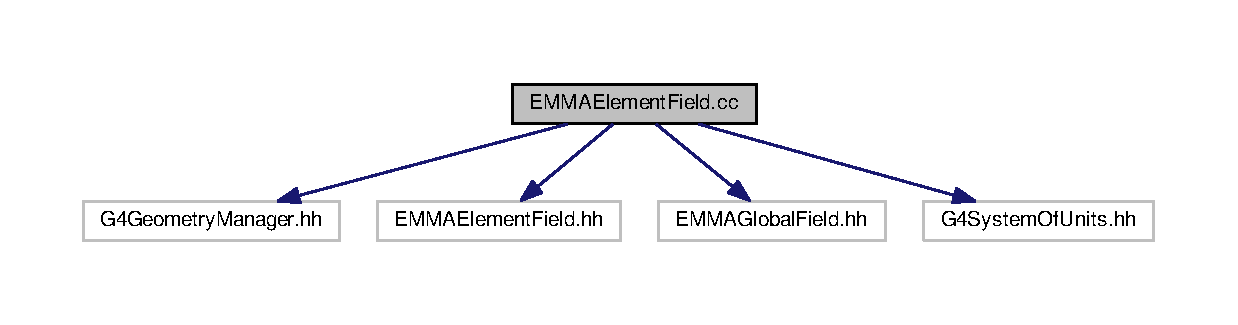
\includegraphics[width=350pt]{EMMAElementField_8cc__incl}
\end{center}
\end{figure}

\hypertarget{EMMAEMPhysics_8cc}{\section{E\-M\-M\-A\-E\-M\-Physics.\-cc File Reference}
\label{EMMAEMPhysics_8cc}\index{E\-M\-M\-A\-E\-M\-Physics.\-cc@{E\-M\-M\-A\-E\-M\-Physics.\-cc}}
}


Defines E\-M physics process functions and particles.  


{\ttfamily \#include \char`\"{}E\-M\-M\-A\-E\-M\-Physics.\-hh\char`\"{}}\\*
{\ttfamily \#include \char`\"{}globals.\-hh\char`\"{}}\\*
{\ttfamily \#include \char`\"{}G4ios.\-hh\char`\"{}}\\*
{\ttfamily \#include $<$iomanip$>$}\\*
{\ttfamily \#include \char`\"{}G4\-Particle\-Definition.\-hh\char`\"{}}\\*
{\ttfamily \#include \char`\"{}G4\-Particle\-Table.\-hh\char`\"{}}\\*
{\ttfamily \#include \char`\"{}G4\-Gamma.\-hh\char`\"{}}\\*
{\ttfamily \#include \char`\"{}G4\-Electron.\-hh\char`\"{}}\\*
{\ttfamily \#include \char`\"{}G4\-Positron.\-hh\char`\"{}}\\*
{\ttfamily \#include \char`\"{}G4\-Neutrino\-E.\-hh\char`\"{}}\\*
{\ttfamily \#include \char`\"{}G4\-Anti\-Neutrino\-E.\-hh\char`\"{}}\\*
{\ttfamily \#include \char`\"{}G4\-Process\-Manager.\-hh\char`\"{}}\\*


\subsection{Detailed Description}
Defines E\-M physics process functions and particles. 
\hypertarget{EMMAEventAction_8cc}{\section{E\-M\-M\-A\-Event\-Action.\-cc File Reference}
\label{EMMAEventAction_8cc}\index{E\-M\-M\-A\-Event\-Action.\-cc@{E\-M\-M\-A\-Event\-Action.\-cc}}
}


Takes care of the interactions (events) of an object that was generated in the Primary Generator. Note\-: If you are getting error messages concerning this file while building E\-M\-M\-A it is likely an error or problem in your (C\-E\-R\-N) R\-O\-O\-T installation, as this file calls upon R\-O\-O\-T functions. Reinstall or remake R\-O\-O\-T, or seek your local computer guru for help.  


{\ttfamily \#include \char`\"{}E\-M\-M\-A\-Event\-Action.\-hh\char`\"{}}\\*
{\ttfamily \#include \char`\"{}E\-M\-M\-A\-Event\-Action\-Messenger.\-hh\char`\"{}}\\*
{\ttfamily \#include \char`\"{}G4\-System\-Of\-Units.\-hh\char`\"{}}\\*
{\ttfamily \#include \char`\"{}G4\-Units\-Table.\-hh\char`\"{}}\\*
{\ttfamily \#include \char`\"{}G4\-Event.\-hh\char`\"{}}\\*
{\ttfamily \#include \char`\"{}G4\-Event\-Manager.\-hh\char`\"{}}\\*
{\ttfamily \#include \char`\"{}G4\-H\-Cof\-This\-Event.\-hh\char`\"{}}\\*
{\ttfamily \#include \char`\"{}G4\-V\-Hits\-Collection.\-hh\char`\"{}}\\*
{\ttfamily \#include \char`\"{}G4\-Trajectory\-Container.\-hh\char`\"{}}\\*
{\ttfamily \#include \char`\"{}G4\-Trajectory.\-hh\char`\"{}}\\*
{\ttfamily \#include \char`\"{}G4\-V\-Vis\-Manager.\-hh\char`\"{}}\\*
{\ttfamily \#include \char`\"{}G4\-S\-D\-Manager.\-hh\char`\"{}}\\*
{\ttfamily \#include \char`\"{}G4\-U\-Imanager.\-hh\char`\"{}}\\*
{\ttfamily \#include \char`\"{}G4ios.\-hh\char`\"{}}\\*
{\ttfamily \#include \char`\"{}E\-M\-M\-A\-Drift\-Chamber\-Hit.\-hh\char`\"{}}\\*
{\ttfamily \#include \char`\"{}E\-M\-M\-A\-Ion\-Chamber.\-hh\char`\"{}}\\*
{\ttfamily \#include \char`\"{}E\-M\-M\-A\-Ion\-Chamber\-Hit.\-hh\char`\"{}}\\*
\subsection*{Variables}
\begin{DoxyCompactItemize}
\item 
\hypertarget{EMMAEventAction_8cc_a8558631b93942e4ae79b3feb21c97c8f}{G4\-String {\bfseries User\-Dir}}\label{EMMAEventAction_8cc_a8558631b93942e4ae79b3feb21c97c8f}

\end{DoxyCompactItemize}


\subsection{Detailed Description}
Takes care of the interactions (events) of an object that was generated in the Primary Generator. Note\-: If you are getting error messages concerning this file while building E\-M\-M\-A it is likely an error or problem in your (C\-E\-R\-N) R\-O\-O\-T installation, as this file calls upon R\-O\-O\-T functions. Reinstall or remake R\-O\-O\-T, or seek your local computer guru for help. 
\hypertarget{EMMAEventActionMessenger_8cc}{}\section{E\+M\+M\+A\+Event\+Action\+Messenger.\+cc File Reference}
\label{EMMAEventActionMessenger_8cc}\index{E\+M\+M\+A\+Event\+Action\+Messenger.\+cc@{E\+M\+M\+A\+Event\+Action\+Messenger.\+cc}}
{\ttfamily \#include \char`\"{}E\+M\+M\+A\+Event\+Action\+Messenger.\+hh\char`\"{}}\\*
{\ttfamily \#include \char`\"{}E\+M\+M\+A\+Event\+Action.\+hh\char`\"{}}\\*
{\ttfamily \#include \char`\"{}G4\+U\+Icmd\+With\+An\+Integer.\+hh\char`\"{}}\\*
{\ttfamily \#include \char`\"{}G4ios.\+hh\char`\"{}}\\*
Include dependency graph for E\+M\+M\+A\+Event\+Action\+Messenger.\+cc\+:
\nopagebreak
\begin{figure}[H]
\begin{center}
\leavevmode
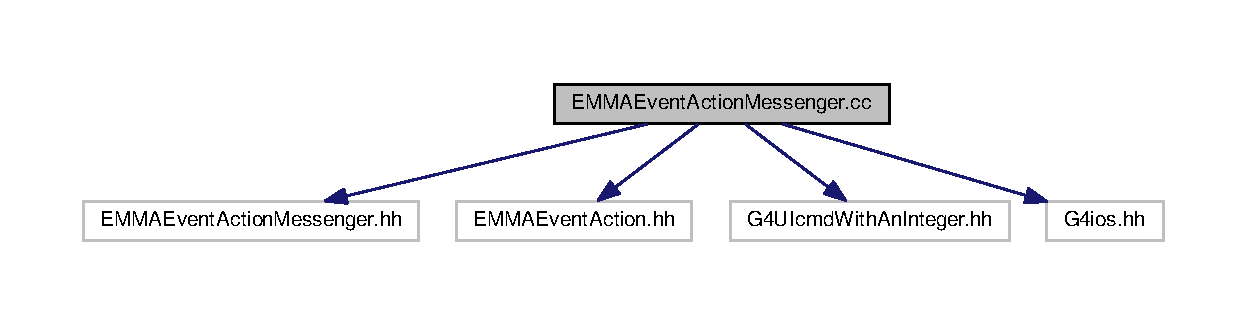
\includegraphics[width=350pt]{EMMAEventActionMessenger_8cc__incl}
\end{center}
\end{figure}

\hypertarget{EMMAGeneralPhysics_8cc}{}\section{E\+M\+M\+A\+General\+Physics.\+cc File Reference}
\label{EMMAGeneralPhysics_8cc}\index{E\+M\+M\+A\+General\+Physics.\+cc@{E\+M\+M\+A\+General\+Physics.\+cc}}
{\ttfamily \#include \char`\"{}E\+M\+M\+A\+General\+Physics.\+hh\char`\"{}}\\*
{\ttfamily \#include \char`\"{}G4\+System\+Of\+Units.\+hh\char`\"{}}\\*
{\ttfamily \#include \char`\"{}globals.\+hh\char`\"{}}\\*
{\ttfamily \#include \char`\"{}G4ios.\+hh\char`\"{}}\\*
{\ttfamily \#include $<$iomanip$>$}\\*
{\ttfamily \#include \char`\"{}F04\+Step\+Max.\+hh\char`\"{}}\\*
{\ttfamily \#include \char`\"{}G4\+Baryon\+Constructor.\+hh\char`\"{}}\\*
{\ttfamily \#include \char`\"{}G4\+Boson\+Constructor.\+hh\char`\"{}}\\*
{\ttfamily \#include \char`\"{}G4\+Ion\+Constructor.\+hh\char`\"{}}\\*
{\ttfamily \#include \char`\"{}G4\+Lepton\+Constructor.\+hh\char`\"{}}\\*
{\ttfamily \#include \char`\"{}G4\+Meson\+Constructor.\+hh\char`\"{}}\\*
{\ttfamily \#include \char`\"{}G4\+Short\+Lived\+Constructor.\+hh\char`\"{}}\\*
{\ttfamily \#include \char`\"{}G4\+Decay.\+hh\char`\"{}}\\*
{\ttfamily \#include \char`\"{}G4\+Particle\+Definition.\+hh\char`\"{}}\\*
{\ttfamily \#include \char`\"{}G4\+Process\+Manager.\+hh\char`\"{}}\\*
{\ttfamily \#include \char`\"{}G4\+Particle\+Table.\+hh\char`\"{}}\\*
{\ttfamily \#include \char`\"{}G4\+V\+User\+Physics\+List.\+hh\char`\"{}}\\*
Include dependency graph for E\+M\+M\+A\+General\+Physics.\+cc\+:
\nopagebreak
\begin{figure}[H]
\begin{center}
\leavevmode
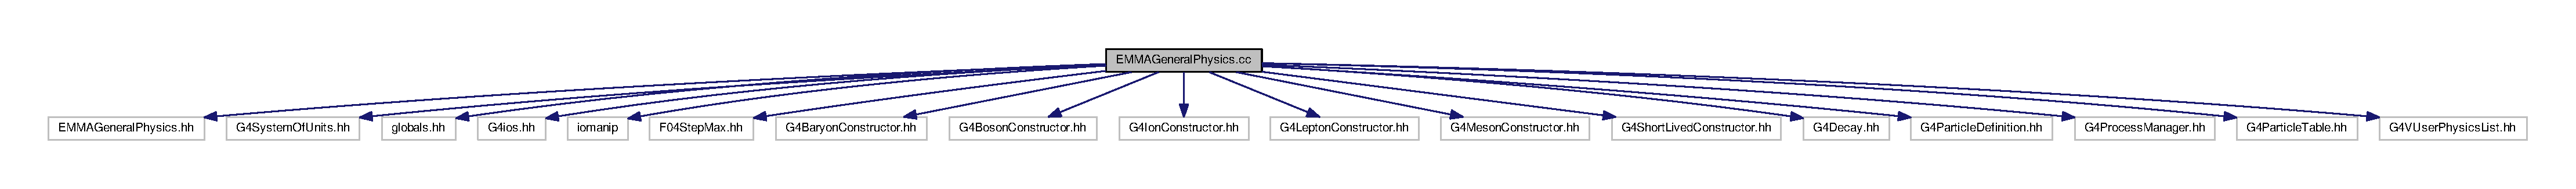
\includegraphics[width=350pt]{EMMAGeneralPhysics_8cc__incl}
\end{center}
\end{figure}

\hypertarget{EMMAGlobalField_8cc}{\section{E\-M\-M\-A\-Global\-Field.\-cc File Reference}
\label{EMMAGlobalField_8cc}\index{E\-M\-M\-A\-Global\-Field.\-cc@{E\-M\-M\-A\-Global\-Field.\-cc}}
}


F04\-Global\-Field -\/ handles the global Electro\-Magnetic field.  


{\ttfamily \#include $<$time.\-h$>$}\\*
{\ttfamily \#include \char`\"{}Randomize.\-hh\char`\"{}}\\*
{\ttfamily \#include \char`\"{}G4\-Transportation\-Manager.\-hh\char`\"{}}\\*
{\ttfamily \#include \char`\"{}G4\-Explicit\-Euler.\-hh\char`\"{}}\\*
{\ttfamily \#include \char`\"{}G4\-Implicit\-Euler.\-hh\char`\"{}}\\*
{\ttfamily \#include \char`\"{}G4\-Simple\-Runge.\-hh\char`\"{}}\\*
{\ttfamily \#include \char`\"{}G4\-Simple\-Heum.\-hh\char`\"{}}\\*
{\ttfamily \#include \char`\"{}G4\-Classical\-R\-K4.\-hh\char`\"{}}\\*
{\ttfamily \#include \char`\"{}G4\-Cash\-Karp\-R\-K\-F45.\-hh\char`\"{}}\\*
{\ttfamily \#include \char`\"{}G4\-System\-Of\-Units.\-hh\char`\"{}}\\*
{\ttfamily \#include \char`\"{}E\-M\-M\-A\-Global\-Field.\-hh\char`\"{}}\\*
{\ttfamily \#include \char`\"{}E\-M\-M\-A\-Element\-Field.\-hh\char`\"{}}\\*
{\ttfamily \#include \char`\"{}E\-M\-Field\-Debugger.\-hh\char`\"{}}\\*


\subsection{Detailed Description}
F04\-Global\-Field -\/ handles the global Electro\-Magnetic field. The field from each individual beamline element (quad, E\-D, etc.) is given by a Element\-Field object. Any number of overlapping Element\-Field objects can be added to the global field. Any element with an E\-M field must add the appropriate Element\-Field to the global Global\-Field object. There is a single G04\-Global\-Field object. 
\hypertarget{EMMAHadronPhysics_8cc}{}\section{E\+M\+M\+A\+Hadron\+Physics.\+cc File Reference}
\label{EMMAHadronPhysics_8cc}\index{E\+M\+M\+A\+Hadron\+Physics.\+cc@{E\+M\+M\+A\+Hadron\+Physics.\+cc}}
{\ttfamily \#include \char`\"{}E\+M\+M\+A\+Hadron\+Physics.\+hh\char`\"{}}\\*
{\ttfamily \#include \char`\"{}globals.\+hh\char`\"{}}\\*
{\ttfamily \#include \char`\"{}G4ios.\+hh\char`\"{}}\\*
{\ttfamily \#include $<$iomanip$>$}\\*
{\ttfamily \#include \char`\"{}G4\+Particle\+Definition.\+hh\char`\"{}}\\*
{\ttfamily \#include \char`\"{}G4\+Particle\+Table.\+hh\char`\"{}}\\*
{\ttfamily \#include \char`\"{}G4\+Process\+Manager.\+hh\char`\"{}}\\*
Include dependency graph for E\+M\+M\+A\+Hadron\+Physics.\+cc\+:
\nopagebreak
\begin{figure}[H]
\begin{center}
\leavevmode
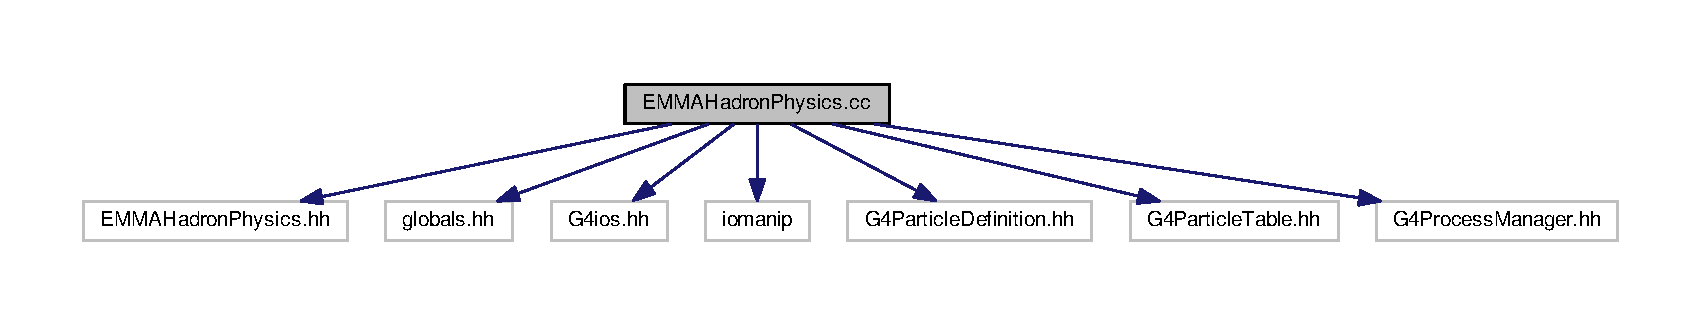
\includegraphics[width=350pt]{EMMAHadronPhysics_8cc__incl}
\end{center}
\end{figure}

\hypertarget{EMMAIonChamber_8cc}{\section{E\-M\-M\-A\-Ion\-Chamber.\-cc File Reference}
\label{EMMAIonChamber_8cc}\index{E\-M\-M\-A\-Ion\-Chamber.\-cc@{E\-M\-M\-A\-Ion\-Chamber.\-cc}}
}


Implementation of the B4c\-Calorimeter\-S\-D class Builds the ion chamber and defines the types of data it outputs. Look here to modify the specific workings of the I\-C. (Look also in Detector\-Construction)  


{\ttfamily \#include \char`\"{}E\-M\-M\-A\-Ion\-Chamber.\-hh\char`\"{}}\\*
{\ttfamily \#include \char`\"{}G4\-H\-Cof\-This\-Event.\-hh\char`\"{}}\\*
{\ttfamily \#include \char`\"{}G4\-Step.\-hh\char`\"{}}\\*
{\ttfamily \#include \char`\"{}G4\-Three\-Vector.\-hh\char`\"{}}\\*
{\ttfamily \#include \char`\"{}G4\-S\-D\-Manager.\-hh\char`\"{}}\\*
{\ttfamily \#include \char`\"{}G4ios.\-hh\char`\"{}}\\*


\subsection{Detailed Description}
Implementation of the B4c\-Calorimeter\-S\-D class Builds the ion chamber and defines the types of data it outputs. Look here to modify the specific workings of the I\-C. (Look also in Detector\-Construction) 
\hypertarget{EMMAIonChamberHit_8cc}{}\section{E\+M\+M\+A\+Ion\+Chamber\+Hit.\+cc File Reference}
\label{EMMAIonChamberHit_8cc}\index{E\+M\+M\+A\+Ion\+Chamber\+Hit.\+cc@{E\+M\+M\+A\+Ion\+Chamber\+Hit.\+cc}}
{\ttfamily \#include \char`\"{}E\+M\+M\+A\+Ion\+Chamber\+Hit.\+hh\char`\"{}}\\*
{\ttfamily \#include \char`\"{}G4\+Units\+Table.\+hh\char`\"{}}\\*
{\ttfamily \#include \char`\"{}G4\+V\+Vis\+Manager.\+hh\char`\"{}}\\*
{\ttfamily \#include \char`\"{}G4\+Circle.\+hh\char`\"{}}\\*
{\ttfamily \#include \char`\"{}G4\+Colour.\+hh\char`\"{}}\\*
{\ttfamily \#include \char`\"{}G4\+Vis\+Attributes.\+hh\char`\"{}}\\*
{\ttfamily \#include $<$iomanip$>$}\\*
Include dependency graph for E\+M\+M\+A\+Ion\+Chamber\+Hit.\+cc\+:
\nopagebreak
\begin{figure}[H]
\begin{center}
\leavevmode
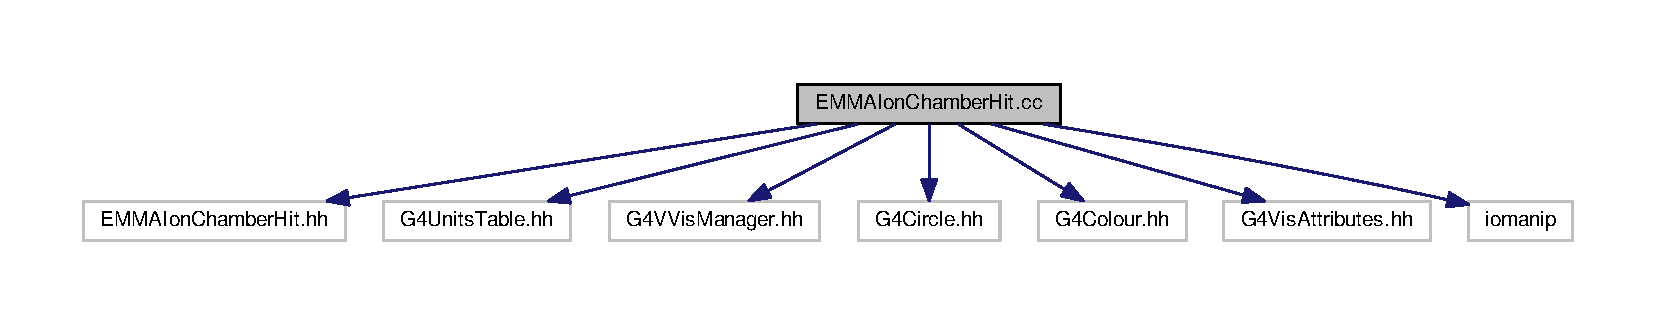
\includegraphics[width=350pt]{EMMAIonChamberHit_8cc__incl}
\end{center}
\end{figure}
\subsection*{Variables}
\begin{DoxyCompactItemize}
\item 
G4\+Allocator$<$ E\+M\+M\+A\+Ion\+Chamber\+Hit $>$ \hyperlink{EMMAIonChamberHit_8cc_adb78e92d0fb21fc2a8a5f8f8d03805ea}{E\+M\+M\+A\+Ion\+Chamber\+Hit\+Allocator}
\end{DoxyCompactItemize}


\subsection{Variable Documentation}
\index{E\+M\+M\+A\+Ion\+Chamber\+Hit.\+cc@{E\+M\+M\+A\+Ion\+Chamber\+Hit.\+cc}!E\+M\+M\+A\+Ion\+Chamber\+Hit\+Allocator@{E\+M\+M\+A\+Ion\+Chamber\+Hit\+Allocator}}
\index{E\+M\+M\+A\+Ion\+Chamber\+Hit\+Allocator@{E\+M\+M\+A\+Ion\+Chamber\+Hit\+Allocator}!E\+M\+M\+A\+Ion\+Chamber\+Hit.\+cc@{E\+M\+M\+A\+Ion\+Chamber\+Hit.\+cc}}
\subsubsection[{\texorpdfstring{E\+M\+M\+A\+Ion\+Chamber\+Hit\+Allocator}{EMMAIonChamberHitAllocator}}]{\setlength{\rightskip}{0pt plus 5cm}G4\+Allocator$<$E\+M\+M\+A\+Ion\+Chamber\+Hit$>$ E\+M\+M\+A\+Ion\+Chamber\+Hit\+Allocator}\hypertarget{EMMAIonChamberHit_8cc_adb78e92d0fb21fc2a8a5f8f8d03805ea}{}\label{EMMAIonChamberHit_8cc_adb78e92d0fb21fc2a8a5f8f8d03805ea}

\hypertarget{EMMAIonPhysics_8cc}{}\section{E\+M\+M\+A\+Ion\+Physics.\+cc File Reference}
\label{EMMAIonPhysics_8cc}\index{E\+M\+M\+A\+Ion\+Physics.\+cc@{E\+M\+M\+A\+Ion\+Physics.\+cc}}
{\ttfamily \#include \char`\"{}E\+M\+M\+A\+Ion\+Physics.\+hh\char`\"{}}\\*
{\ttfamily \#include \char`\"{}globals.\+hh\char`\"{}}\\*
{\ttfamily \#include \char`\"{}G4ios.\+hh\char`\"{}}\\*
{\ttfamily \#include $<$iomanip$>$}\\*
{\ttfamily \#include \char`\"{}G4\+Region.\+hh\char`\"{}}\\*
{\ttfamily \#include \char`\"{}G4\+Region\+Store.\+hh\char`\"{}}\\*
{\ttfamily \#include \char`\"{}G4\+Production\+Cuts.\+hh\char`\"{}}\\*
{\ttfamily \#include \char`\"{}G4\+Em\+Configurator.\+hh\char`\"{}}\\*
{\ttfamily \#include \char`\"{}G4\+Loss\+Table\+Manager.\+hh\char`\"{}}\\*
{\ttfamily \#include \char`\"{}G4\+Bragg\+Ion\+Gas\+Model.\+hh\char`\"{}}\\*
{\ttfamily \#include \char`\"{}G4\+Bethe\+Bloch\+Ion\+Gas\+Model.\+hh\char`\"{}}\\*
{\ttfamily \#include \char`\"{}G4\+Ion\+Fluctuations.\+hh\char`\"{}}\\*
{\ttfamily \#include \char`\"{}G4\+Universal\+Fluctuation.\+hh\char`\"{}}\\*
{\ttfamily \#include \char`\"{}G4\+Particle\+Definition.\+hh\char`\"{}}\\*
{\ttfamily \#include \char`\"{}G4\+Particle\+Table.\+hh\char`\"{}}\\*
{\ttfamily \#include \char`\"{}G4\+Process\+Manager.\+hh\char`\"{}}\\*
{\ttfamily \#include \char`\"{}G4\+Em\+Process\+Options.\+hh\char`\"{}}\\*
{\ttfamily \#include \char`\"{}G4\+Ion\+Parametrised\+Loss\+Model.\+hh\char`\"{}}\\*
{\ttfamily \#include \char`\"{}G4\+Nuclear\+Stopping.\+hh\char`\"{}}\\*
{\ttfamily \#include \char`\"{}G4\+Urban\+Msc\+Model90.\+hh\char`\"{}}\\*
{\ttfamily \#include \char`\"{}G4\+Urban\+Msc\+Model95.\+hh\char`\"{}}\\*
{\ttfamily \#include \char`\"{}G4\+Wentzel\+V\+I\+Model.\+hh\char`\"{}}\\*
{\ttfamily \#include \char`\"{}G4\+Coulomb\+Scattering.\+hh\char`\"{}}\\*
{\ttfamily \#include \char`\"{}G4\+Ion\+Coulomb\+Scattering\+Model.\+hh\char`\"{}}\\*
{\ttfamily \#include \char`\"{}G4\+Screened\+Nuclear\+Recoil.\+hh\char`\"{}}\\*
{\ttfamily \#include \char`\"{}E\+M\+M\+A\+Ion\+Physics\+Messenger.\+hh\char`\"{}}\\*
Include dependency graph for E\+M\+M\+A\+Ion\+Physics.\+cc\+:
\nopagebreak
\begin{figure}[H]
\begin{center}
\leavevmode
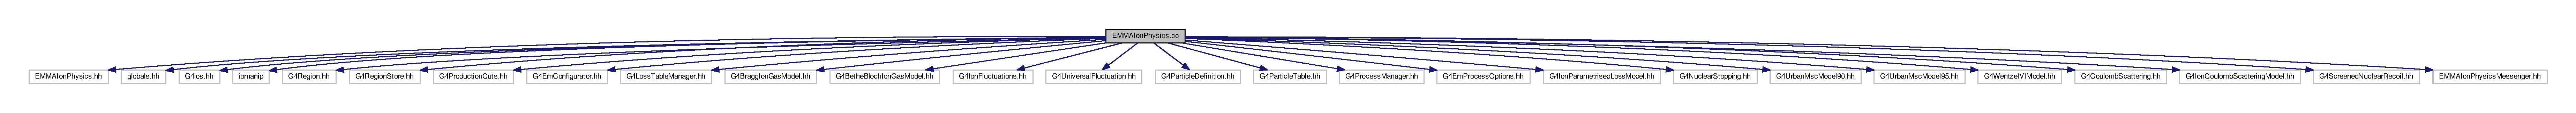
\includegraphics[width=350pt]{EMMAIonPhysics_8cc__incl}
\end{center}
\end{figure}

\hypertarget{EMMAIonPhysicsMessenger_8cc}{\section{E\-M\-M\-A\-Ion\-Physics\-Messenger.\-cc File Reference}
\label{EMMAIonPhysicsMessenger_8cc}\index{E\-M\-M\-A\-Ion\-Physics\-Messenger.\-cc@{E\-M\-M\-A\-Ion\-Physics\-Messenger.\-cc}}
}


Connects and delivers user commands regarding ion physics particles and processes to respective classes, and relays their responses to the user.  


{\ttfamily \#include \char`\"{}E\-M\-M\-A\-Ion\-Physics\-Messenger.\-hh\char`\"{}}\\*
{\ttfamily \#include \char`\"{}E\-M\-M\-A\-Ion\-Physics.\-hh\char`\"{}}\\*
{\ttfamily \#include \char`\"{}G4\-U\-Icmd\-With\-A\-Double\-And\-Unit.\-hh\char`\"{}}\\*
{\ttfamily \#include \char`\"{}G4\-U\-Icmd\-With\-A\-Double.\-hh\char`\"{}}\\*
{\ttfamily \#include \char`\"{}G4\-U\-Icmd\-With\-A\-Bool.\-hh\char`\"{}}\\*
{\ttfamily \#include \char`\"{}G4ios.\-hh\char`\"{}}\\*


\subsection{Detailed Description}
Connects and delivers user commands regarding ion physics particles and processes to respective classes, and relays their responses to the user. 
\hypertarget{EMMAMuonPhysics_8cc}{}\section{E\+M\+M\+A\+Muon\+Physics.\+cc File Reference}
\label{EMMAMuonPhysics_8cc}\index{E\+M\+M\+A\+Muon\+Physics.\+cc@{E\+M\+M\+A\+Muon\+Physics.\+cc}}
{\ttfamily \#include \char`\"{}E\+M\+M\+A\+Muon\+Physics.\+hh\char`\"{}}\\*
{\ttfamily \#include \char`\"{}globals.\+hh\char`\"{}}\\*
{\ttfamily \#include \char`\"{}G4ios.\+hh\char`\"{}}\\*
{\ttfamily \#include $<$iomanip$>$}\\*
{\ttfamily \#include \char`\"{}G4\+Particle\+Definition.\+hh\char`\"{}}\\*
{\ttfamily \#include \char`\"{}G4\+Particle\+Table.\+hh\char`\"{}}\\*
{\ttfamily \#include \char`\"{}G4\+Muon\+Plus.\+hh\char`\"{}}\\*
{\ttfamily \#include \char`\"{}G4\+Muon\+Minus.\+hh\char`\"{}}\\*
{\ttfamily \#include \char`\"{}G4\+Tau\+Minus.\+hh\char`\"{}}\\*
{\ttfamily \#include \char`\"{}G4\+Tau\+Plus.\+hh\char`\"{}}\\*
{\ttfamily \#include \char`\"{}G4\+Process\+Manager.\+hh\char`\"{}}\\*
Include dependency graph for E\+M\+M\+A\+Muon\+Physics.\+cc\+:
\nopagebreak
\begin{figure}[H]
\begin{center}
\leavevmode
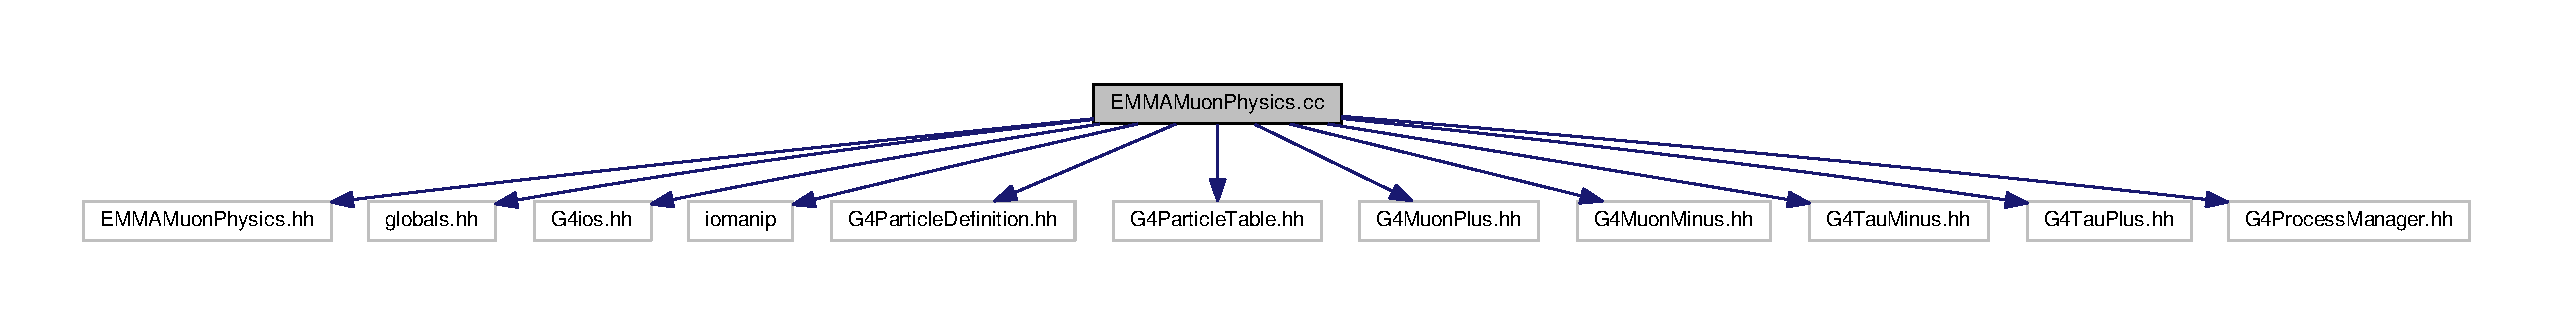
\includegraphics[width=350pt]{EMMAMuonPhysics_8cc__incl}
\end{center}
\end{figure}

\hypertarget{EMMANuclearReactionDataSet_8cc}{}\section{E\+M\+M\+A\+Nuclear\+Reaction\+Data\+Set.\+cc File Reference}
\label{EMMANuclearReactionDataSet_8cc}\index{E\+M\+M\+A\+Nuclear\+Reaction\+Data\+Set.\+cc@{E\+M\+M\+A\+Nuclear\+Reaction\+Data\+Set.\+cc}}
{\ttfamily \#include \char`\"{}G4\+Nist\+Manager.\+hh\char`\"{}}\\*
{\ttfamily \#include \char`\"{}G4\+Had\+Tmp\+Util.\+hh\char`\"{}}\\*
{\ttfamily \#include $<$iostream$>$}\\*
{\ttfamily \#include \char`\"{}E\+M\+M\+A\+Nuclear\+Reaction\+Data\+Set.\+hh\char`\"{}}\\*
Include dependency graph for E\+M\+M\+A\+Nuclear\+Reaction\+Data\+Set.\+cc\+:
\nopagebreak
\begin{figure}[H]
\begin{center}
\leavevmode
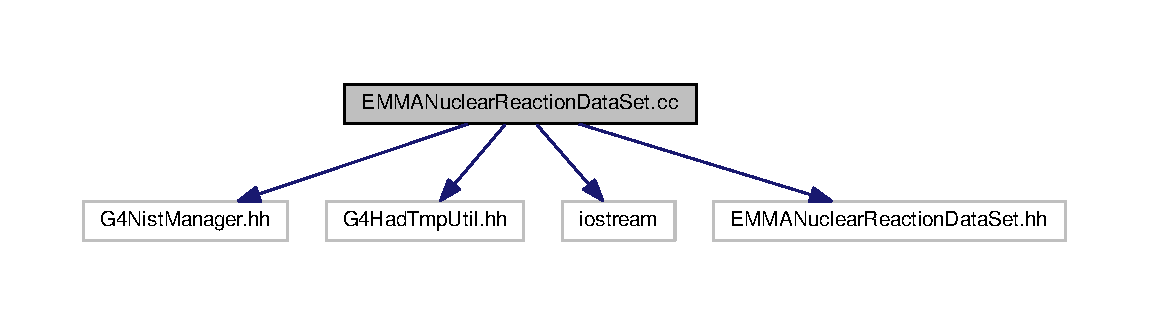
\includegraphics[width=350pt]{EMMANuclearReactionDataSet_8cc__incl}
\end{center}
\end{figure}

\hypertarget{EMMANuclearReactionProcess_8cc}{}\section{E\+M\+M\+A\+Nuclear\+Reaction\+Process.\+cc File Reference}
\label{EMMANuclearReactionProcess_8cc}\index{E\+M\+M\+A\+Nuclear\+Reaction\+Process.\+cc@{E\+M\+M\+A\+Nuclear\+Reaction\+Process.\+cc}}
{\ttfamily \#include $<$iostream$>$}\\*
{\ttfamily \#include $<$typeinfo$>$}\\*
{\ttfamily \#include \char`\"{}G4\+System\+Of\+Units.\+hh\char`\"{}}\\*
{\ttfamily \#include \char`\"{}G4\+Nucleus.\+hh\char`\"{}}\\*
{\ttfamily \#include \char`\"{}G4\+Process\+Manager.\+hh\char`\"{}}\\*
{\ttfamily \#include \char`\"{}G4\+Cross\+Section\+Data\+Store.\+hh\char`\"{}}\\*
{\ttfamily \#include \char`\"{}E\+M\+M\+A\+Nuclear\+Reaction\+Data\+Set.\+hh\char`\"{}}\\*
{\ttfamily \#include \char`\"{}G4\+Production\+Cuts\+Table.\+hh\char`\"{}}\\*
{\ttfamily \#include \char`\"{}G4\+Hadronic\+Exception.\+hh\char`\"{}}\\*
{\ttfamily \#include \char`\"{}G4\+Hadronic\+Deprecate.\+hh\char`\"{}}\\*
{\ttfamily \#include \char`\"{}E\+M\+M\+A\+Nuclear\+Reaction\+Process.\+hh\char`\"{}}\\*
{\ttfamily \#include \char`\"{}E\+M\+M\+A\+Nuclear\+Reaction\+Two\+Body.\+hh\char`\"{}}\\*
Include dependency graph for E\+M\+M\+A\+Nuclear\+Reaction\+Process.\+cc\+:
\nopagebreak
\begin{figure}[H]
\begin{center}
\leavevmode
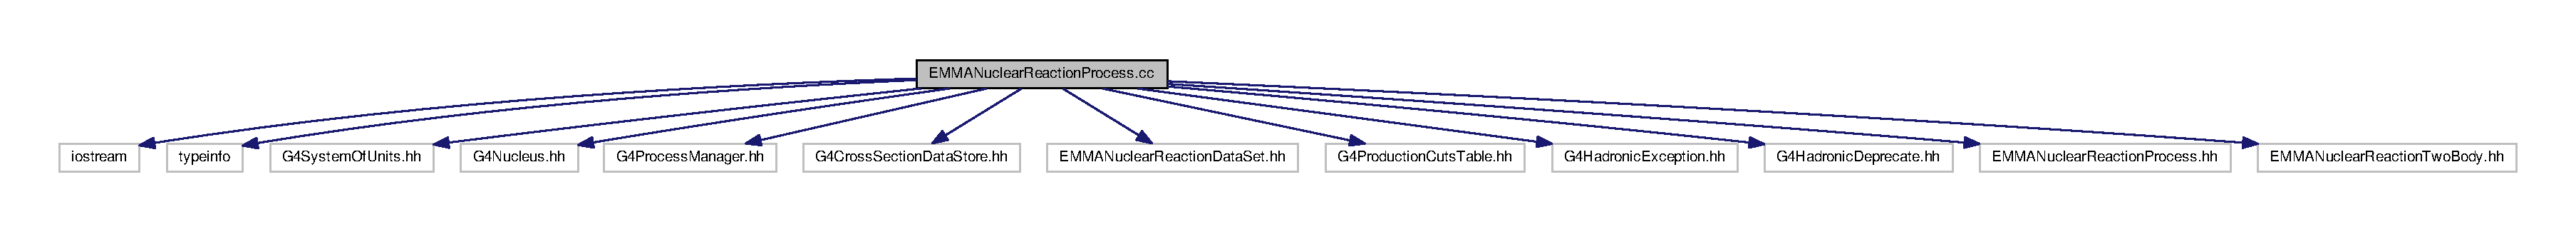
\includegraphics[width=350pt]{EMMANuclearReactionProcess_8cc__incl}
\end{center}
\end{figure}

\hypertarget{EMMANuclearReactionTwoBody_8cc}{}\section{E\+M\+M\+A\+Nuclear\+Reaction\+Two\+Body.\+cc File Reference}
\label{EMMANuclearReactionTwoBody_8cc}\index{E\+M\+M\+A\+Nuclear\+Reaction\+Two\+Body.\+cc@{E\+M\+M\+A\+Nuclear\+Reaction\+Two\+Body.\+cc}}
{\ttfamily \#include $<$iostream$>$}\\*
{\ttfamily \#include \char`\"{}E\+M\+M\+A\+Nuclear\+Reaction\+Two\+Body.\+hh\char`\"{}}\\*
{\ttfamily \#include \char`\"{}globals.\+hh\char`\"{}}\\*
{\ttfamily \#include \char`\"{}G4\+Physical\+Constants.\+hh\char`\"{}}\\*
{\ttfamily \#include \char`\"{}G4\+System\+Of\+Units.\+hh\char`\"{}}\\*
{\ttfamily \#include \char`\"{}Randomize.\+hh\char`\"{}}\\*
{\ttfamily \#include \char`\"{}G4\+Particle\+Table.\+hh\char`\"{}}\\*
{\ttfamily \#include \char`\"{}G4\+Ion\+Table.\+hh\char`\"{}}\\*
{\ttfamily \#include \char`\"{}G4\+Proton.\+hh\char`\"{}}\\*
{\ttfamily \#include \char`\"{}G4\+Neutron.\+hh\char`\"{}}\\*
{\ttfamily \#include \char`\"{}G4\+Deuteron.\+hh\char`\"{}}\\*
{\ttfamily \#include \char`\"{}G4\+Triton.\+hh\char`\"{}}\\*
{\ttfamily \#include \char`\"{}G4\+Alpha.\+hh\char`\"{}}\\*
{\ttfamily \#include \char`\"{}G4\+He3.\+hh\char`\"{}}\\*
{\ttfamily \#include \char`\"{}G4\+Gamma.\+hh\char`\"{}}\\*
{\ttfamily \#include \char`\"{}G4\+Nuclei\+Properties.\+hh\char`\"{}}\\*
Include dependency graph for E\+M\+M\+A\+Nuclear\+Reaction\+Two\+Body.\+cc\+:
\nopagebreak
\begin{figure}[H]
\begin{center}
\leavevmode
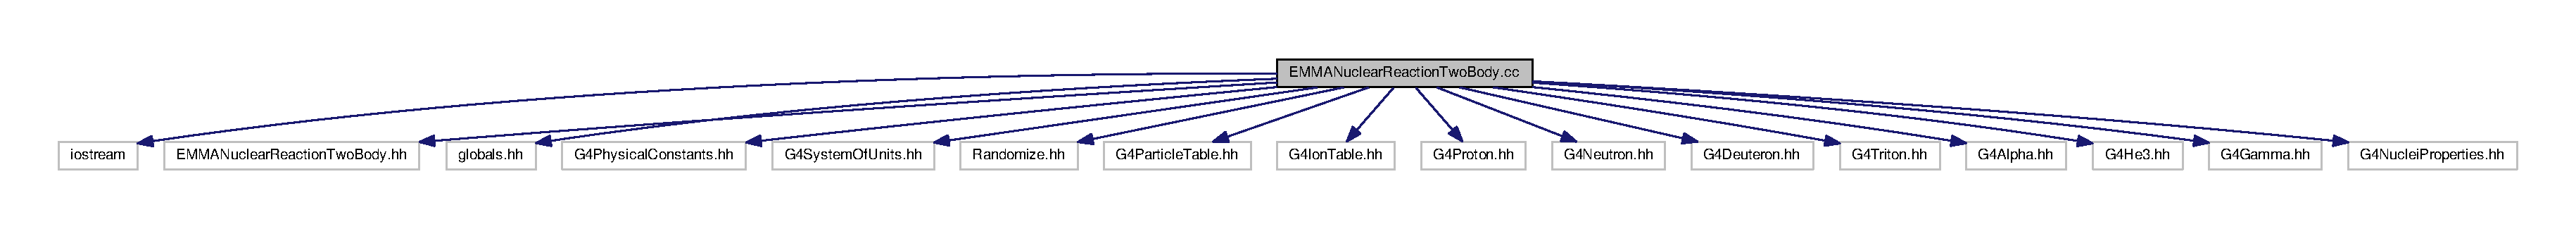
\includegraphics[width=350pt]{EMMANuclearReactionTwoBody_8cc__incl}
\end{center}
\end{figure}

\hypertarget{EMMAPhysicsList_8cc}{}\section{E\+M\+M\+A\+Physics\+List.\+cc File Reference}
\label{EMMAPhysicsList_8cc}\index{E\+M\+M\+A\+Physics\+List.\+cc@{E\+M\+M\+A\+Physics\+List.\+cc}}
{\ttfamily \#include \char`\"{}E\+M\+M\+A\+Physics\+List.\+hh\char`\"{}}\\*
{\ttfamily \#include \char`\"{}globals.\+hh\char`\"{}}\\*
{\ttfamily \#include \char`\"{}G4\+Particle\+Definition.\+hh\char`\"{}}\\*
{\ttfamily \#include \char`\"{}G4\+Particle\+With\+Cuts.\+hh\char`\"{}}\\*
{\ttfamily \#include \char`\"{}G4\+Process\+Manager.\+hh\char`\"{}}\\*
{\ttfamily \#include \char`\"{}G4\+Process\+Vector.\+hh\char`\"{}}\\*
{\ttfamily \#include \char`\"{}G4\+Particle\+Types.\+hh\char`\"{}}\\*
{\ttfamily \#include \char`\"{}G4\+Particle\+Table.\+hh\char`\"{}}\\*
{\ttfamily \#include \char`\"{}G4\+Material.\+hh\char`\"{}}\\*
{\ttfamily \#include \char`\"{}G4\+Material\+Table.\+hh\char`\"{}}\\*
{\ttfamily \#include \char`\"{}G4ios.\+hh\char`\"{}}\\*
{\ttfamily \#include $<$iomanip$>$}\\*
{\ttfamily \#include \char`\"{}E\+M\+M\+A\+General\+Physics.\+hh\char`\"{}}\\*
{\ttfamily \#include \char`\"{}E\+M\+M\+A\+E\+M\+Physics.\+hh\char`\"{}}\\*
{\ttfamily \#include \char`\"{}E\+M\+M\+A\+Muon\+Physics.\+hh\char`\"{}}\\*
{\ttfamily \#include \char`\"{}E\+M\+M\+A\+Hadron\+Physics.\+hh\char`\"{}}\\*
{\ttfamily \#include \char`\"{}E\+M\+M\+A\+Ion\+Physics.\+hh\char`\"{}}\\*
Include dependency graph for E\+M\+M\+A\+Physics\+List.\+cc\+:
\nopagebreak
\begin{figure}[H]
\begin{center}
\leavevmode
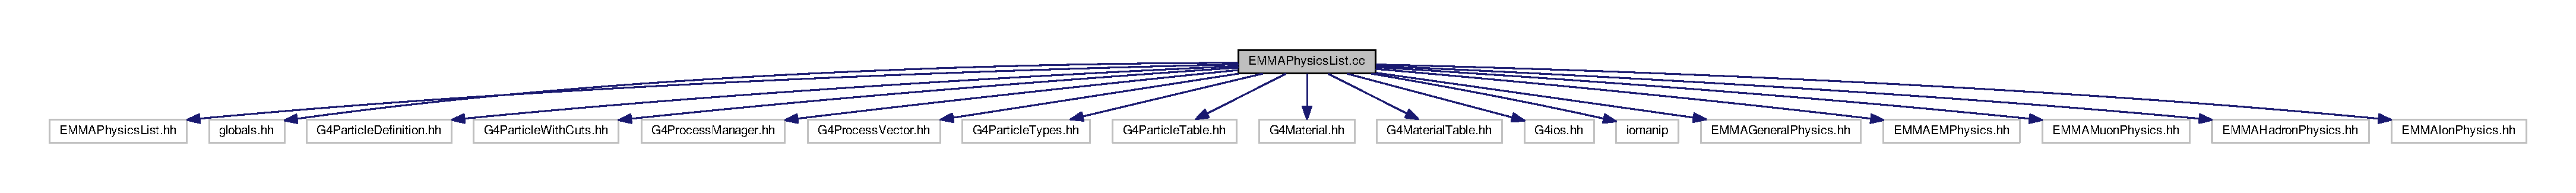
\includegraphics[width=350pt]{EMMAPhysicsList_8cc__incl}
\end{center}
\end{figure}

\hypertarget{EMMAPrimaryGeneratorAction_8cc}{}\section{E\+M\+M\+A\+Primary\+Generator\+Action.\+cc File Reference}
\label{EMMAPrimaryGeneratorAction_8cc}\index{E\+M\+M\+A\+Primary\+Generator\+Action.\+cc@{E\+M\+M\+A\+Primary\+Generator\+Action.\+cc}}
{\ttfamily \#include \char`\"{}E\+M\+M\+A\+Primary\+Generator\+Action.\+hh\char`\"{}}\\*
{\ttfamily \#include \char`\"{}E\+M\+M\+A\+Primary\+Generator\+Messenger.\+hh\char`\"{}}\\*
{\ttfamily \#include \char`\"{}G4\+Event.\+hh\char`\"{}}\\*
{\ttfamily \#include \char`\"{}G4\+Particle\+Gun.\+hh\char`\"{}}\\*
{\ttfamily \#include \char`\"{}G4\+Particle\+Table.\+hh\char`\"{}}\\*
{\ttfamily \#include \char`\"{}G4\+Particle\+Definition.\+hh\char`\"{}}\\*
{\ttfamily \#include \char`\"{}Randomize.\+hh\char`\"{}}\\*
{\ttfamily \#include \char`\"{}G4ios.\+hh\char`\"{}}\\*
{\ttfamily \#include \char`\"{}G4\+Units\+Table.\+hh\char`\"{}}\\*
{\ttfamily \#include \char`\"{}G4\+Track.\+hh\char`\"{}}\\*
{\ttfamily \#include \char`\"{}G4\+Step.\+hh\char`\"{}}\\*
{\ttfamily \#include \char`\"{}G4\+Particle\+Types.\+hh\char`\"{}}\\*
{\ttfamily \#include \char`\"{}G4\+Physical\+Constants.\+hh\char`\"{}}\\*
{\ttfamily \#include \char`\"{}G4\+System\+Of\+Units.\+hh\char`\"{}}\\*
{\ttfamily \#include \char`\"{}G4\+Ion\+Table.\+hh\char`\"{}}\\*
{\ttfamily \#include \char`\"{}G4\+Nuclei\+Properties.\+hh\char`\"{}}\\*
{\ttfamily \#include \char`\"{}G4\+Gamma.\+hh\char`\"{}}\\*
{\ttfamily \#include \char`\"{}G4\+Run\+Manager.\+hh\char`\"{}}\\*
{\ttfamily \#include \char`\"{}G4\+Logical\+Volume\+Store.\+hh\char`\"{}}\\*
{\ttfamily \#include \char`\"{}G4\+Logical\+Volume.\+hh\char`\"{}}\\*
{\ttfamily \#include \char`\"{}G4\+V\+Solid.\+hh\char`\"{}}\\*
{\ttfamily \#include \char`\"{}G4\+Box.\+hh\char`\"{}}\\*
{\ttfamily \#include $<$string$>$}\\*
{\ttfamily \#include $<$fstream$>$}\\*
{\ttfamily \#include $<$sstream$>$}\\*
Include dependency graph for E\+M\+M\+A\+Primary\+Generator\+Action.\+cc\+:
\nopagebreak
\begin{figure}[H]
\begin{center}
\leavevmode
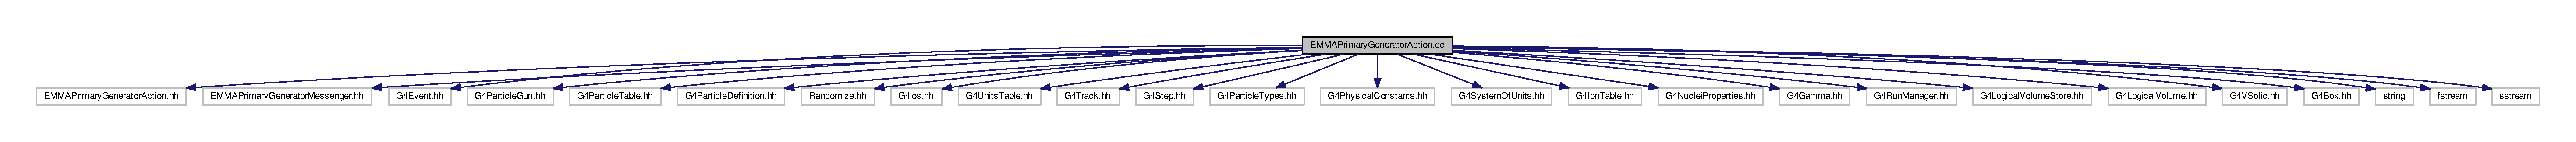
\includegraphics[width=350pt]{EMMAPrimaryGeneratorAction_8cc__incl}
\end{center}
\end{figure}
\subsection*{Variables}
\begin{DoxyCompactItemize}
\item 
G4bool \hyperlink{EMMAPrimaryGeneratorAction_8cc_accd97970a0ee52817a02f8bdf0969668}{prepare\+Beam} = true
\item 
G4\+String \hyperlink{EMMAPrimaryGeneratorAction_8cc_ab5043f10e6a2b6521cf9bdc5f9b50a14}{in\+Target\+File\+Name}
\item 
G4\+String \hyperlink{EMMAPrimaryGeneratorAction_8cc_a44c8e472e5202caa69e70c5e8d18adf7}{post\+Target\+File\+Name}
\item 
G4\+String \hyperlink{EMMAPrimaryGeneratorAction_8cc_a3dbaf7156a8d958508b9806a0ef50aa6}{focal\+Plane\+File\+Name}
\item 
G4double \hyperlink{EMMAPrimaryGeneratorAction_8cc_a2d61cdd1b1b5ed409f7c91b54737c1b9}{user\+Charge} = 54.
\item 
G4\+String \hyperlink{EMMAPrimaryGeneratorAction_8cc_ae92d83921bde0242f8c619b79b457b23}{post\+Degrader1\+File\+Name}
\item 
G4double \hyperlink{EMMAPrimaryGeneratorAction_8cc_a08a40c9f48981a0140f43cbf773f3eea}{depth}
\end{DoxyCompactItemize}


\subsection{Variable Documentation}
\index{E\+M\+M\+A\+Primary\+Generator\+Action.\+cc@{E\+M\+M\+A\+Primary\+Generator\+Action.\+cc}!depth@{depth}}
\index{depth@{depth}!E\+M\+M\+A\+Primary\+Generator\+Action.\+cc@{E\+M\+M\+A\+Primary\+Generator\+Action.\+cc}}
\subsubsection[{\texorpdfstring{depth}{depth}}]{\setlength{\rightskip}{0pt plus 5cm}G4double depth}\hypertarget{EMMAPrimaryGeneratorAction_8cc_a08a40c9f48981a0140f43cbf773f3eea}{}\label{EMMAPrimaryGeneratorAction_8cc_a08a40c9f48981a0140f43cbf773f3eea}
\index{E\+M\+M\+A\+Primary\+Generator\+Action.\+cc@{E\+M\+M\+A\+Primary\+Generator\+Action.\+cc}!focal\+Plane\+File\+Name@{focal\+Plane\+File\+Name}}
\index{focal\+Plane\+File\+Name@{focal\+Plane\+File\+Name}!E\+M\+M\+A\+Primary\+Generator\+Action.\+cc@{E\+M\+M\+A\+Primary\+Generator\+Action.\+cc}}
\subsubsection[{\texorpdfstring{focal\+Plane\+File\+Name}{focalPlaneFileName}}]{\setlength{\rightskip}{0pt plus 5cm}G4\+String focal\+Plane\+File\+Name}\hypertarget{EMMAPrimaryGeneratorAction_8cc_a3dbaf7156a8d958508b9806a0ef50aa6}{}\label{EMMAPrimaryGeneratorAction_8cc_a3dbaf7156a8d958508b9806a0ef50aa6}
\index{E\+M\+M\+A\+Primary\+Generator\+Action.\+cc@{E\+M\+M\+A\+Primary\+Generator\+Action.\+cc}!in\+Target\+File\+Name@{in\+Target\+File\+Name}}
\index{in\+Target\+File\+Name@{in\+Target\+File\+Name}!E\+M\+M\+A\+Primary\+Generator\+Action.\+cc@{E\+M\+M\+A\+Primary\+Generator\+Action.\+cc}}
\subsubsection[{\texorpdfstring{in\+Target\+File\+Name}{inTargetFileName}}]{\setlength{\rightskip}{0pt plus 5cm}G4\+String in\+Target\+File\+Name}\hypertarget{EMMAPrimaryGeneratorAction_8cc_ab5043f10e6a2b6521cf9bdc5f9b50a14}{}\label{EMMAPrimaryGeneratorAction_8cc_ab5043f10e6a2b6521cf9bdc5f9b50a14}
\index{E\+M\+M\+A\+Primary\+Generator\+Action.\+cc@{E\+M\+M\+A\+Primary\+Generator\+Action.\+cc}!post\+Degrader1\+File\+Name@{post\+Degrader1\+File\+Name}}
\index{post\+Degrader1\+File\+Name@{post\+Degrader1\+File\+Name}!E\+M\+M\+A\+Primary\+Generator\+Action.\+cc@{E\+M\+M\+A\+Primary\+Generator\+Action.\+cc}}
\subsubsection[{\texorpdfstring{post\+Degrader1\+File\+Name}{postDegrader1FileName}}]{\setlength{\rightskip}{0pt plus 5cm}G4\+String post\+Degrader1\+File\+Name}\hypertarget{EMMAPrimaryGeneratorAction_8cc_ae92d83921bde0242f8c619b79b457b23}{}\label{EMMAPrimaryGeneratorAction_8cc_ae92d83921bde0242f8c619b79b457b23}
\index{E\+M\+M\+A\+Primary\+Generator\+Action.\+cc@{E\+M\+M\+A\+Primary\+Generator\+Action.\+cc}!post\+Target\+File\+Name@{post\+Target\+File\+Name}}
\index{post\+Target\+File\+Name@{post\+Target\+File\+Name}!E\+M\+M\+A\+Primary\+Generator\+Action.\+cc@{E\+M\+M\+A\+Primary\+Generator\+Action.\+cc}}
\subsubsection[{\texorpdfstring{post\+Target\+File\+Name}{postTargetFileName}}]{\setlength{\rightskip}{0pt plus 5cm}G4\+String post\+Target\+File\+Name}\hypertarget{EMMAPrimaryGeneratorAction_8cc_a44c8e472e5202caa69e70c5e8d18adf7}{}\label{EMMAPrimaryGeneratorAction_8cc_a44c8e472e5202caa69e70c5e8d18adf7}
\index{E\+M\+M\+A\+Primary\+Generator\+Action.\+cc@{E\+M\+M\+A\+Primary\+Generator\+Action.\+cc}!prepare\+Beam@{prepare\+Beam}}
\index{prepare\+Beam@{prepare\+Beam}!E\+M\+M\+A\+Primary\+Generator\+Action.\+cc@{E\+M\+M\+A\+Primary\+Generator\+Action.\+cc}}
\subsubsection[{\texorpdfstring{prepare\+Beam}{prepareBeam}}]{\setlength{\rightskip}{0pt plus 5cm}G4bool prepare\+Beam = true}\hypertarget{EMMAPrimaryGeneratorAction_8cc_accd97970a0ee52817a02f8bdf0969668}{}\label{EMMAPrimaryGeneratorAction_8cc_accd97970a0ee52817a02f8bdf0969668}
\index{E\+M\+M\+A\+Primary\+Generator\+Action.\+cc@{E\+M\+M\+A\+Primary\+Generator\+Action.\+cc}!user\+Charge@{user\+Charge}}
\index{user\+Charge@{user\+Charge}!E\+M\+M\+A\+Primary\+Generator\+Action.\+cc@{E\+M\+M\+A\+Primary\+Generator\+Action.\+cc}}
\subsubsection[{\texorpdfstring{user\+Charge}{userCharge}}]{\setlength{\rightskip}{0pt plus 5cm}G4double user\+Charge = 54.}\hypertarget{EMMAPrimaryGeneratorAction_8cc_a2d61cdd1b1b5ed409f7c91b54737c1b9}{}\label{EMMAPrimaryGeneratorAction_8cc_a2d61cdd1b1b5ed409f7c91b54737c1b9}

\hypertarget{EMMAPrimaryGeneratorMessenger_8cc}{\section{E\-M\-M\-A\-Primary\-Generator\-Messenger.\-cc File Reference}
\label{EMMAPrimaryGeneratorMessenger_8cc}\index{E\-M\-M\-A\-Primary\-Generator\-Messenger.\-cc@{E\-M\-M\-A\-Primary\-Generator\-Messenger.\-cc}}
}


Connects and delivers user commands regarding the primary generator actions to respective classes, and relays their responses.  


{\ttfamily \#include \char`\"{}E\-M\-M\-A\-Primary\-Generator\-Messenger.\-hh\char`\"{}}\\*
{\ttfamily \#include \char`\"{}E\-M\-M\-A\-Primary\-Generator\-Action.\-hh\char`\"{}}\\*
{\ttfamily \#include \char`\"{}G4\-U\-Icmd\-With\-A\-Double\-And\-Unit.\-hh\char`\"{}}\\*
{\ttfamily \#include \char`\"{}G4\-U\-Icmd\-With\-A\-Bool.\-hh\char`\"{}}\\*
{\ttfamily \#include \char`\"{}G4\-U\-Icmd\-With\-A\-Double.\-hh\char`\"{}}\\*
{\ttfamily \#include \char`\"{}G4\-U\-Icmd\-With\-An\-Integer.\-hh\char`\"{}}\\*
{\ttfamily \#include \char`\"{}G4ios.\-hh\char`\"{}}\\*


\subsection{Detailed Description}
Connects and delivers user commands regarding the primary generator actions to respective classes, and relays their responses. 
\hypertarget{EMMASteppingAction_8cc}{\section{E\-M\-M\-A\-Stepping\-Action.\-cc File Reference}
\label{EMMASteppingAction_8cc}\index{E\-M\-M\-A\-Stepping\-Action.\-cc@{E\-M\-M\-A\-Stepping\-Action.\-cc}}
}


Tracks the particle as it makes its way through the spectrometer. Ensures that the beam projectiles do not pass through the target. Writes beam information as it passes through target so a collision can be simulated. Records and writes the locations of (dead) hits to a R\-O\-O\-T histogram.  


{\ttfamily \#include \char`\"{}E\-M\-M\-A\-Stepping\-Action.\-hh\char`\"{}}\\*
{\ttfamily \#include \char`\"{}E\-M\-M\-A\-Global\-Field.\-hh\char`\"{}}\\*
{\ttfamily \#include \char`\"{}E\-M\-M\-A\-Element\-Field.\-hh\char`\"{}}\\*
{\ttfamily \#include \char`\"{}G4\-Stepping\-Manager.\-hh\char`\"{}}\\*
{\ttfamily \#include \char`\"{}G4\-Track.\-hh\char`\"{}}\\*
{\ttfamily \#include \char`\"{}G4\-Step.\-hh\char`\"{}}\\*
{\ttfamily \#include \char`\"{}G4\-Step\-Point.\-hh\char`\"{}}\\*
{\ttfamily \#include \char`\"{}G4\-Track\-Status.\-hh\char`\"{}}\\*
{\ttfamily \#include \char`\"{}G4\-V\-Physical\-Volume.\-hh\char`\"{}}\\*
{\ttfamily \#include \char`\"{}G4\-Particle\-Definition.\-hh\char`\"{}}\\*
{\ttfamily \#include \char`\"{}G4\-Particle\-Types.\-hh\char`\"{}}\\*
{\ttfamily \#include \char`\"{}G4\-Touchable\-Handle.\-hh\char`\"{}}\\*
{\ttfamily \#include \char`\"{}G4\-Event\-Manager.\-hh\char`\"{}}\\*
{\ttfamily \#include \char`\"{}G4\-Run\-Manager.\-hh\char`\"{}}\\*
{\ttfamily \#include \char`\"{}G4\-Units\-Table.\-hh\char`\"{}}\\*
{\ttfamily \#include $<$G4\-Event.\-hh$>$}\\*
\subsection*{Variables}
\begin{DoxyCompactItemize}
\item 
\hypertarget{EMMASteppingAction_8cc_acb265d8eecfa1acd31056f0c7915362e}{G4double {\bfseries current\-Charge} = 0.\-0}\label{EMMASteppingAction_8cc_acb265d8eecfa1acd31056f0c7915362e}

\end{DoxyCompactItemize}


\subsection{Detailed Description}
Tracks the particle as it makes its way through the spectrometer. Ensures that the beam projectiles do not pass through the target. Writes beam information as it passes through target so a collision can be simulated. Records and writes the locations of (dead) hits to a R\-O\-O\-T histogram. 
\hypertarget{EMMASteppingVerbose_8cc}{\section{E\-M\-M\-A\-Stepping\-Verbose.\-cc File Reference}
\label{EMMASteppingVerbose_8cc}\index{E\-M\-M\-A\-Stepping\-Verbose.\-cc@{E\-M\-M\-A\-Stepping\-Verbose.\-cc}}
}


Prints out the information obtained in Stepping\-Action (Hence verbose).  


{\ttfamily \#include \char`\"{}E\-M\-M\-A\-Stepping\-Verbose.\-hh\char`\"{}}\\*
{\ttfamily \#include \char`\"{}G4\-Stepping\-Manager.\-hh\char`\"{}}\\*
{\ttfamily \#include \char`\"{}G4\-Units\-Table.\-hh\char`\"{}}\\*


\subsection{Detailed Description}
Prints out the information obtained in Stepping\-Action (Hence verbose). 
\hypertarget{F04StepMax_8cc}{}\section{F04\+Step\+Max.\+cc File Reference}
\label{F04StepMax_8cc}\index{F04\+Step\+Max.\+cc@{F04\+Step\+Max.\+cc}}
{\ttfamily \#include \char`\"{}G4\+Track.\+hh\char`\"{}}\\*
{\ttfamily \#include \char`\"{}G4\+V\+Particle\+Change.\+hh\char`\"{}}\\*
{\ttfamily \#include \char`\"{}F04\+Step\+Max.\+hh\char`\"{}}\\*
Include dependency graph for F04\+Step\+Max.\+cc\+:
\nopagebreak
\begin{figure}[H]
\begin{center}
\leavevmode
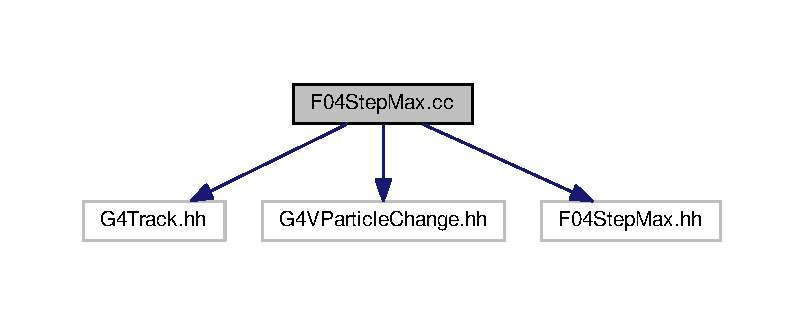
\includegraphics[width=350pt]{F04StepMax_8cc__incl}
\end{center}
\end{figure}

\hypertarget{G4LindhardPartition_8cc}{}\section{G4\+Lindhard\+Partition.\+cc File Reference}
\label{G4LindhardPartition_8cc}\index{G4\+Lindhard\+Partition.\+cc@{G4\+Lindhard\+Partition.\+cc}}
{\ttfamily \#include \char`\"{}G4\+Lindhard\+Partition.\+hh\char`\"{}}\\*
{\ttfamily \#include \char`\"{}G4\+Material.\+hh\char`\"{}}\\*
{\ttfamily \#include \char`\"{}G4\+Element.\+hh\char`\"{}}\\*
{\ttfamily \#include \char`\"{}G4\+Physical\+Constants.\+hh\char`\"{}}\\*
{\ttfamily \#include \char`\"{}G4\+System\+Of\+Units.\+hh\char`\"{}}\\*
Include dependency graph for G4\+Lindhard\+Partition.\+cc\+:
\nopagebreak
\begin{figure}[H]
\begin{center}
\leavevmode
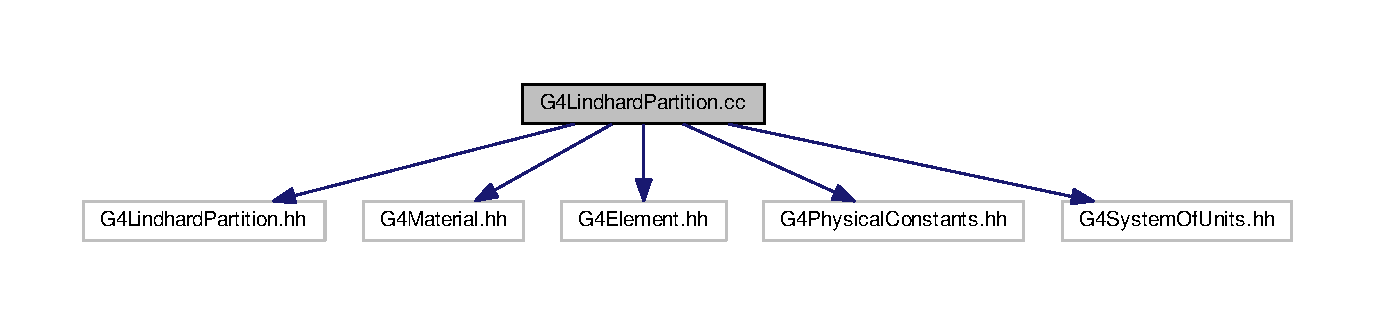
\includegraphics[width=350pt]{G4LindhardPartition_8cc__incl}
\end{center}
\end{figure}

\hypertarget{G4ScreenedNuclearRecoil_8cc}{\section{G4\-Screened\-Nuclear\-Recoil.\-cc File Reference}
\label{G4ScreenedNuclearRecoil_8cc}\index{G4\-Screened\-Nuclear\-Recoil.\-cc@{G4\-Screened\-Nuclear\-Recoil.\-cc}}
}


Implementation of the G4\-Screened\-Nuclear\-Recoil class Process for screened electromagnetic nuclear elastic scattering;.  


{\ttfamily \#include $<$stdio.\-h$>$}\\*
{\ttfamily \#include \char`\"{}globals.\-hh\char`\"{}}\\*
{\ttfamily \#include \char`\"{}G4\-Screened\-Nuclear\-Recoil.\-hh\char`\"{}}\\*
{\ttfamily \#include \char`\"{}G4\-Particle\-Types.\-hh\char`\"{}}\\*
{\ttfamily \#include \char`\"{}G4\-Particle\-Table.\-hh\char`\"{}}\\*
{\ttfamily \#include \char`\"{}G4\-V\-Particle\-Change.\-hh\char`\"{}}\\*
{\ttfamily \#include \char`\"{}G4\-Particle\-Change\-For\-Loss.\-hh\char`\"{}}\\*
{\ttfamily \#include \char`\"{}G4\-Data\-Vector.\-hh\char`\"{}}\\*
{\ttfamily \#include \char`\"{}G4\-Track.\-hh\char`\"{}}\\*
{\ttfamily \#include \char`\"{}G4\-Step.\-hh\char`\"{}}\\*
{\ttfamily \#include \char`\"{}G4\-Material.\-hh\char`\"{}}\\*
{\ttfamily \#include \char`\"{}G4\-Element.\-hh\char`\"{}}\\*
{\ttfamily \#include \char`\"{}G4\-Isotope.\-hh\char`\"{}}\\*
{\ttfamily \#include \char`\"{}G4\-Material\-Cuts\-Couple.\-hh\char`\"{}}\\*
{\ttfamily \#include \char`\"{}G4\-Element\-Vector.\-hh\char`\"{}}\\*
{\ttfamily \#include \char`\"{}G4\-Isotope\-Vector.\-hh\char`\"{}}\\*
{\ttfamily \#include \char`\"{}G4\-Em\-Process\-Sub\-Type.\-hh\char`\"{}}\\*
{\ttfamily \#include \char`\"{}G4\-Range\-Test.\-hh\char`\"{}}\\*
{\ttfamily \#include \char`\"{}G4\-Particle\-Definition.\-hh\char`\"{}}\\*
{\ttfamily \#include \char`\"{}G4\-Dynamic\-Particle.\-hh\char`\"{}}\\*
{\ttfamily \#include \char`\"{}G4\-Process\-Manager.\-hh\char`\"{}}\\*
{\ttfamily \#include \char`\"{}G4\-Stable\-Isotopes.\-hh\char`\"{}}\\*
{\ttfamily \#include \char`\"{}G4\-Lindhard\-Partition.\-hh\char`\"{}}\\*
{\ttfamily \#include \char`\"{}G4\-Physical\-Constants.\-hh\char`\"{}}\\*
{\ttfamily \#include \char`\"{}G4\-System\-Of\-Units.\-hh\char`\"{}}\\*
{\ttfamily \#include \char`\"{}Randomize.\-hh\char`\"{}}\\*
{\ttfamily \#include $<$iostream$>$}\\*
{\ttfamily \#include $<$iomanip$>$}\\*
{\ttfamily \#include \char`\"{}c2\-\_\-factory.\-hh\char`\"{}}\\*
{\ttfamily \#include $<$vector$>$}\\*
\subsection*{Typedefs}
\begin{DoxyCompactItemize}
\item 
\hypertarget{G4ScreenedNuclearRecoil_8cc_a6c336ea4b7120ec7a7ed097d8865b4b7}{typedef c2\-\_\-ptr$<$ G4double $>$ {\bfseries c2p}}\label{G4ScreenedNuclearRecoil_8cc_a6c336ea4b7120ec7a7ed097d8865b4b7}

\end{DoxyCompactItemize}
\subsection*{Functions}
\begin{DoxyCompactItemize}
\item 
\hypertarget{G4ScreenedNuclearRecoil_8cc_a38390a6f2bb8ba250affdccb1c9cc49c}{G4\-\_\-c2\-\_\-function \& {\bfseries Z\-B\-L\-Screening} (G4int z1, G4int z2, size\-\_\-t npoints, G4double r\-Max, G4double $\ast$auval)}\label{G4ScreenedNuclearRecoil_8cc_a38390a6f2bb8ba250affdccb1c9cc49c}

\item 
\hypertarget{G4ScreenedNuclearRecoil_8cc_af83b8ddfa7c0df319b4573c74bb4afd3}{G4\-\_\-c2\-\_\-function \& {\bfseries Moliere\-Screening} (G4int z1, G4int z2, size\-\_\-t npoints, G4double r\-Max, G4double $\ast$auval)}\label{G4ScreenedNuclearRecoil_8cc_af83b8ddfa7c0df319b4573c74bb4afd3}

\item 
\hypertarget{G4ScreenedNuclearRecoil_8cc_afab442d2da9f659d2c7d4b9bb1e64f5e}{G4\-\_\-c2\-\_\-function \& {\bfseries L\-J\-Screening} (G4int z1, G4int z2, size\-\_\-t npoints, G4double r\-Max, G4double $\ast$auval)}\label{G4ScreenedNuclearRecoil_8cc_afab442d2da9f659d2c7d4b9bb1e64f5e}

\item 
\hypertarget{G4ScreenedNuclearRecoil_8cc_a1e2dbe4b8a87ad052a14e6c21ad98cbf}{G4\-\_\-c2\-\_\-function \& {\bfseries L\-J\-Z\-B\-L\-Screening} (G4int z1, G4int z2, size\-\_\-t npoints, G4double r\-Max, G4double $\ast$auval)}\label{G4ScreenedNuclearRecoil_8cc_a1e2dbe4b8a87ad052a14e6c21ad98cbf}

\end{DoxyCompactItemize}


\subsection{Detailed Description}
Implementation of the G4\-Screened\-Nuclear\-Recoil class Process for screened electromagnetic nuclear elastic scattering;. See this file for more detailed in-\/body description and reference. 
\hypertarget{SpectrometerConstruction_8cc}{}\section{Spectrometer\+Construction.\+cc File Reference}
\label{SpectrometerConstruction_8cc}\index{Spectrometer\+Construction.\+cc@{Spectrometer\+Construction.\+cc}}
{\ttfamily \#include \char`\"{}Spectrometer\+Construction.\+hh\char`\"{}}\\*
{\ttfamily \#include \char`\"{}G4\+V\+Solid.\+hh\char`\"{}}\\*
{\ttfamily \#include \char`\"{}G4\+Box.\+hh\char`\"{}}\\*
{\ttfamily \#include \char`\"{}G4\+Tubs.\+hh\char`\"{}}\\*
{\ttfamily \#include \char`\"{}G4\+Logical\+Volume.\+hh\char`\"{}}\\*
{\ttfamily \#include \char`\"{}G4\+V\+Physical\+Volume.\+hh\char`\"{}}\\*
{\ttfamily \#include \char`\"{}G4\+P\+V\+Placement.\+hh\char`\"{}}\\*
{\ttfamily \#include \char`\"{}G4\+Production\+Cuts\+Table.\+hh\char`\"{}}\\*
{\ttfamily \#include \char`\"{}E\+M\+M\+A\+Global\+Field.\+hh\char`\"{}}\\*
{\ttfamily \#include \char`\"{}E\+M\+Field\+Debugger.\+hh\char`\"{}}\\*
{\ttfamily \#include \char`\"{}G4\+Vis\+Attributes.\+hh\char`\"{}}\\*
{\ttfamily \#include \char`\"{}G4\+Colour.\+hh\char`\"{}}\\*
{\ttfamily \#include \char`\"{}G4\+Region.\+hh\char`\"{}}\\*
{\ttfamily \#include \char`\"{}G4\+Union\+Solid.\+hh\char`\"{}}\\*
{\ttfamily \#include \char`\"{}G4\+Region\+Store.\+hh\char`\"{}}\\*
{\ttfamily \#include \char`\"{}G4\+User\+Limits.\+hh\char`\"{}}\\*
{\ttfamily \#include \char`\"{}G4\+Material.\+hh\char`\"{}}\\*
{\ttfamily \#include \char`\"{}G4\+Material\+Table.\+hh\char`\"{}}\\*
{\ttfamily \#include \char`\"{}G4\+Element.\+hh\char`\"{}}\\*
{\ttfamily \#include \char`\"{}G4\+Units\+Table.\+hh\char`\"{}}\\*
{\ttfamily \#include \char`\"{}G4\+Transform3\+D.\+hh\char`\"{}}\\*
{\ttfamily \#include $<$fstream$>$}\\*
{\ttfamily \#include $<$stdlib.\+h$>$}\\*
{\ttfamily \#include \char`\"{}B\+G\+Field1.\+hh\char`\"{}}\\*
{\ttfamily \#include \char`\"{}B\+G\+Field2.\+hh\char`\"{}}\\*
{\ttfamily \#include \char`\"{}B\+G\+Field3.\+hh\char`\"{}}\\*
{\ttfamily \#include \char`\"{}B\+G\+Field4.\+hh\char`\"{}}\\*
{\ttfamily \#include \char`\"{}B\+G\+Field5.\+hh\char`\"{}}\\*
{\ttfamily \#include \char`\"{}B\+G\+Field6.\+hh\char`\"{}}\\*
{\ttfamily \#include \char`\"{}B\+G\+Field7.\+hh\char`\"{}}\\*
Include dependency graph for Spectrometer\+Construction.\+cc\+:
\nopagebreak
\begin{figure}[H]
\begin{center}
\leavevmode
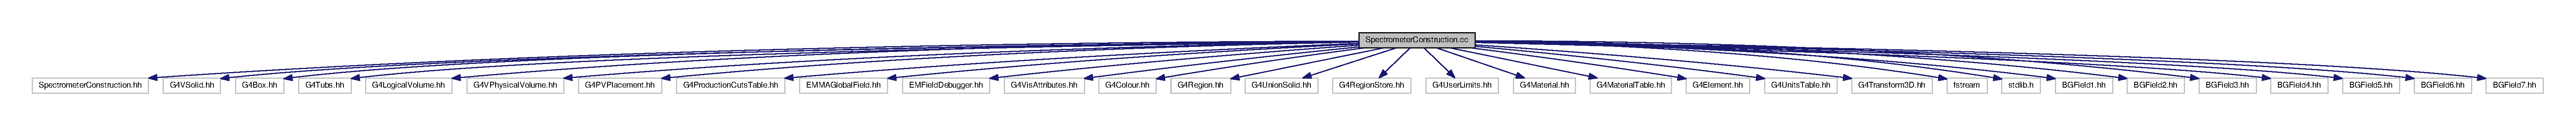
\includegraphics[width=350pt]{SpectrometerConstruction_8cc__incl}
\end{center}
\end{figure}
\subsection*{Variables}
\begin{DoxyCompactItemize}
\item 
G4double \hyperlink{SpectrometerConstruction_8cc_a63b4d37f848ab857400025988ebc68ac}{z\+Q1begins}
\item 
G4double \hyperlink{SpectrometerConstruction_8cc_aaefdf69418ceee3aabc72a346eef1799}{z\+Q4ends}
\item 
G4double \hyperlink{SpectrometerConstruction_8cc_a9906ccfd8985bb28a72c37e7cd16f277}{z\+Anode}
\item 
G4double \hyperlink{SpectrometerConstruction_8cc_a499096b9dc56ffa559bd1aec0bafe28e}{z\+Focal\+Plane}
\item 
G4double \hyperlink{SpectrometerConstruction_8cc_a8825e4bac9c627d0fc56ceb808baee99}{z\+Q1ends}
\item 
G4double \hyperlink{SpectrometerConstruction_8cc_a0389aed4a205ff7970a9c57db9776625}{z\+Q2ends}
\item 
G4double \hyperlink{SpectrometerConstruction_8cc_aa309293d04a3e9edd55505001bb8842f}{z\+Q3ends}
\item 
G4double \hyperlink{SpectrometerConstruction_8cc_a62d0de84d7d6b0923e982b354afad285}{z\+Q2begins}
\item 
G4double \hyperlink{SpectrometerConstruction_8cc_a12daa717eecd47b0ce06c1314040fc3c}{z\+Q3begins}
\item 
G4double \hyperlink{SpectrometerConstruction_8cc_ab2b8c71527a18e35d81eb8bd6e7691f4}{z\+Q4begins}
\item 
G4double \hyperlink{SpectrometerConstruction_8cc_aad92ec801d3e4699e64b73238d977d97}{z\+Q1fieldbegins}
\item 
G4double \hyperlink{SpectrometerConstruction_8cc_a312fb44f7507d957ccc70c34d5d94a43}{z\+Q2fieldbegins}
\item 
G4double \hyperlink{SpectrometerConstruction_8cc_a92fc8c51d58e20801f34d52f8a2c7a2b}{z\+Q2fieldends}
\item 
G4double \hyperlink{SpectrometerConstruction_8cc_a077f13a115281633166d7450d5f26fa0}{z\+Q3fieldbegins}
\item 
G4double \hyperlink{SpectrometerConstruction_8cc_afb3a8a6427088f204ef91b7361831904}{z\+Q4fieldbegins}
\item 
G4double \hyperlink{SpectrometerConstruction_8cc_a2f06aa9a2a32a33fa1100ce176ab4636}{z\+Q4fieldends}
\item 
G4double \hyperlink{SpectrometerConstruction_8cc_a3feee11b7c51f66f2b05335422fd6766}{z\+E\+D1fieldbegins}
\item 
G4double \hyperlink{SpectrometerConstruction_8cc_ab9ae78ef340f126ece97727282006616}{x\+E\+D1fieldends}
\item 
G4double \hyperlink{SpectrometerConstruction_8cc_a233a000653cf27b6f9124c2a55731df1}{z\+E\+D1fieldends}
\item 
G4double \hyperlink{SpectrometerConstruction_8cc_a20f1012cd491461a26923d2c5e7bf9e9}{x\+M\+Dfieldbegins}
\item 
G4double \hyperlink{SpectrometerConstruction_8cc_a69783c655a650a2d465aa29adb99becd}{z\+M\+Dfieldbegins}
\item 
G4double \hyperlink{SpectrometerConstruction_8cc_a159fc7800979fa9630bfc45a7f78596c}{x\+M\+Dfieldends}
\item 
G4double \hyperlink{SpectrometerConstruction_8cc_ac69dbd129f1b938df9976d51f7593e8d}{z\+M\+Dfieldends}
\item 
G4double \hyperlink{SpectrometerConstruction_8cc_a1756cc9671bdb5e3fef3244359b6d3cc}{x\+E\+D2fieldbegins}
\item 
G4double \hyperlink{SpectrometerConstruction_8cc_ad016826f85af9d76258e59348edeb364}{z\+E\+D2fieldbegins}
\item 
G4double \hyperlink{SpectrometerConstruction_8cc_a9d0bd55552fe4d1f2f44f49d35cc081e}{z\+E\+D2fieldends}
\item 
G4double \hyperlink{SpectrometerConstruction_8cc_a244d4cfe9b2fed8a950b5260924858ff}{x\+E\+D1center}
\item 
G4double \hyperlink{SpectrometerConstruction_8cc_a74ebfc53f3a93114f6d28295ee4ab9f4}{z\+E\+D1center}
\item 
G4double \hyperlink{SpectrometerConstruction_8cc_a3c58a920166faad49e1879314c55c5be}{x\+E\+D2center}
\item 
G4double \hyperlink{SpectrometerConstruction_8cc_ac98e44690840a121652fcb08b156a635}{z\+E\+D2center}
\item 
G4double \hyperlink{SpectrometerConstruction_8cc_a715d053d73470185e7c2c4702d9dc2de}{r\+ED}
\item 
G4double \hyperlink{SpectrometerConstruction_8cc_aebdd7edbdb400c898923e8d3722725bf}{x\+M\+Dcenter}
\item 
G4double \hyperlink{SpectrometerConstruction_8cc_ac5e70ecd77b70fb29053de3d744defbe}{z\+M\+Dcenter}
\item 
G4double \hyperlink{SpectrometerConstruction_8cc_a7fd4fbedfa36308277282111f3a02a2e}{r\+MD}
\item 
G4double \hyperlink{SpectrometerConstruction_8cc_a6a82266fb838ffa86812c6000c9dc287}{Q1before}
\item 
G4double \hyperlink{SpectrometerConstruction_8cc_a5566ea3bf099349decdfcf3c26fc376c}{Q2before}
\item 
G4double \hyperlink{SpectrometerConstruction_8cc_a75fe85cecce8dd0b8fa08cf97cee4ce2}{E\+D1before}
\item 
G4double \hyperlink{SpectrometerConstruction_8cc_a003204f9438882eab89ba42ae5708f37}{M\+Dbefore}
\item 
G4double \hyperlink{SpectrometerConstruction_8cc_a1fb2ee29034baaf6ed6e2acbdbf8b578}{E\+D2before}
\item 
G4double \hyperlink{SpectrometerConstruction_8cc_a2fe0c19691575193f51b8ef4c4301aad}{Q3before}
\item 
G4double \hyperlink{SpectrometerConstruction_8cc_a807b9ab7f57ec0c8bdc7764053d3e516}{Q4before}
\item 
G4double \hyperlink{SpectrometerConstruction_8cc_a79e8de762c55f46eaf341c33ddcdfabd}{Q1after}
\item 
G4double \hyperlink{SpectrometerConstruction_8cc_a9d33b4b693d4f7341602ab26cb44359c}{Q2after}
\item 
G4double \hyperlink{SpectrometerConstruction_8cc_a56c3dd0f81ddd6f90cfcc044fb51dff1}{E\+D1after}
\item 
G4double \hyperlink{SpectrometerConstruction_8cc_af04f7784a3cdd89375e6c74b915d255c}{M\+Dafter}
\item 
G4double \hyperlink{SpectrometerConstruction_8cc_ad4c429af59f2e7eee31d1480df299599}{E\+D2after}
\item 
G4double \hyperlink{SpectrometerConstruction_8cc_a7a55e4b1397f5859cde14aa271bb3717}{Q3after}
\item 
G4double \hyperlink{SpectrometerConstruction_8cc_a47d7897cbc13a67cc420cfb3ec97fd60}{Q4after}
\item 
G4double \hyperlink{SpectrometerConstruction_8cc_a58acf77da23d6d58252d729d4d8212d1}{Pipe4z}
\item 
G4double \hyperlink{SpectrometerConstruction_8cc_ab20b3e8fa2797e410fb9110cfad39796}{Pipe4\+HL}
\item 
G4double \hyperlink{SpectrometerConstruction_8cc_a7369eeb2c228d92eeb2a6e7ad496e13f}{Pipe7\+HL}
\item 
G4\+String \hyperlink{SpectrometerConstruction_8cc_ae9b14cfeccc31b1bf76af2f4c3aae43d}{field\+File\+Name}
\item 
G4\+String \hyperlink{SpectrometerConstruction_8cc_a8558631b93942e4ae79b3feb21c97c8f}{User\+Dir}
\end{DoxyCompactItemize}


\subsection{Variable Documentation}
\index{Spectrometer\+Construction.\+cc@{Spectrometer\+Construction.\+cc}!E\+D1after@{E\+D1after}}
\index{E\+D1after@{E\+D1after}!Spectrometer\+Construction.\+cc@{Spectrometer\+Construction.\+cc}}
\subsubsection[{\texorpdfstring{E\+D1after}{ED1after}}]{\setlength{\rightskip}{0pt plus 5cm}G4double E\+D1after}\hypertarget{SpectrometerConstruction_8cc_a56c3dd0f81ddd6f90cfcc044fb51dff1}{}\label{SpectrometerConstruction_8cc_a56c3dd0f81ddd6f90cfcc044fb51dff1}
\index{Spectrometer\+Construction.\+cc@{Spectrometer\+Construction.\+cc}!E\+D1before@{E\+D1before}}
\index{E\+D1before@{E\+D1before}!Spectrometer\+Construction.\+cc@{Spectrometer\+Construction.\+cc}}
\subsubsection[{\texorpdfstring{E\+D1before}{ED1before}}]{\setlength{\rightskip}{0pt plus 5cm}G4double E\+D1before}\hypertarget{SpectrometerConstruction_8cc_a75fe85cecce8dd0b8fa08cf97cee4ce2}{}\label{SpectrometerConstruction_8cc_a75fe85cecce8dd0b8fa08cf97cee4ce2}
\index{Spectrometer\+Construction.\+cc@{Spectrometer\+Construction.\+cc}!E\+D2after@{E\+D2after}}
\index{E\+D2after@{E\+D2after}!Spectrometer\+Construction.\+cc@{Spectrometer\+Construction.\+cc}}
\subsubsection[{\texorpdfstring{E\+D2after}{ED2after}}]{\setlength{\rightskip}{0pt plus 5cm}G4double E\+D2after}\hypertarget{SpectrometerConstruction_8cc_ad4c429af59f2e7eee31d1480df299599}{}\label{SpectrometerConstruction_8cc_ad4c429af59f2e7eee31d1480df299599}
\index{Spectrometer\+Construction.\+cc@{Spectrometer\+Construction.\+cc}!E\+D2before@{E\+D2before}}
\index{E\+D2before@{E\+D2before}!Spectrometer\+Construction.\+cc@{Spectrometer\+Construction.\+cc}}
\subsubsection[{\texorpdfstring{E\+D2before}{ED2before}}]{\setlength{\rightskip}{0pt plus 5cm}G4double E\+D2before}\hypertarget{SpectrometerConstruction_8cc_a1fb2ee29034baaf6ed6e2acbdbf8b578}{}\label{SpectrometerConstruction_8cc_a1fb2ee29034baaf6ed6e2acbdbf8b578}
\index{Spectrometer\+Construction.\+cc@{Spectrometer\+Construction.\+cc}!field\+File\+Name@{field\+File\+Name}}
\index{field\+File\+Name@{field\+File\+Name}!Spectrometer\+Construction.\+cc@{Spectrometer\+Construction.\+cc}}
\subsubsection[{\texorpdfstring{field\+File\+Name}{fieldFileName}}]{\setlength{\rightskip}{0pt plus 5cm}G4\+String field\+File\+Name}\hypertarget{SpectrometerConstruction_8cc_ae9b14cfeccc31b1bf76af2f4c3aae43d}{}\label{SpectrometerConstruction_8cc_ae9b14cfeccc31b1bf76af2f4c3aae43d}
\index{Spectrometer\+Construction.\+cc@{Spectrometer\+Construction.\+cc}!M\+Dafter@{M\+Dafter}}
\index{M\+Dafter@{M\+Dafter}!Spectrometer\+Construction.\+cc@{Spectrometer\+Construction.\+cc}}
\subsubsection[{\texorpdfstring{M\+Dafter}{MDafter}}]{\setlength{\rightskip}{0pt plus 5cm}G4double M\+Dafter}\hypertarget{SpectrometerConstruction_8cc_af04f7784a3cdd89375e6c74b915d255c}{}\label{SpectrometerConstruction_8cc_af04f7784a3cdd89375e6c74b915d255c}
\index{Spectrometer\+Construction.\+cc@{Spectrometer\+Construction.\+cc}!M\+Dbefore@{M\+Dbefore}}
\index{M\+Dbefore@{M\+Dbefore}!Spectrometer\+Construction.\+cc@{Spectrometer\+Construction.\+cc}}
\subsubsection[{\texorpdfstring{M\+Dbefore}{MDbefore}}]{\setlength{\rightskip}{0pt plus 5cm}G4double M\+Dbefore}\hypertarget{SpectrometerConstruction_8cc_a003204f9438882eab89ba42ae5708f37}{}\label{SpectrometerConstruction_8cc_a003204f9438882eab89ba42ae5708f37}
\index{Spectrometer\+Construction.\+cc@{Spectrometer\+Construction.\+cc}!Pipe4\+HL@{Pipe4\+HL}}
\index{Pipe4\+HL@{Pipe4\+HL}!Spectrometer\+Construction.\+cc@{Spectrometer\+Construction.\+cc}}
\subsubsection[{\texorpdfstring{Pipe4\+HL}{Pipe4HL}}]{\setlength{\rightskip}{0pt plus 5cm}G4double Pipe4\+HL}\hypertarget{SpectrometerConstruction_8cc_ab20b3e8fa2797e410fb9110cfad39796}{}\label{SpectrometerConstruction_8cc_ab20b3e8fa2797e410fb9110cfad39796}
\index{Spectrometer\+Construction.\+cc@{Spectrometer\+Construction.\+cc}!Pipe4z@{Pipe4z}}
\index{Pipe4z@{Pipe4z}!Spectrometer\+Construction.\+cc@{Spectrometer\+Construction.\+cc}}
\subsubsection[{\texorpdfstring{Pipe4z}{Pipe4z}}]{\setlength{\rightskip}{0pt plus 5cm}G4double Pipe4z}\hypertarget{SpectrometerConstruction_8cc_a58acf77da23d6d58252d729d4d8212d1}{}\label{SpectrometerConstruction_8cc_a58acf77da23d6d58252d729d4d8212d1}
\index{Spectrometer\+Construction.\+cc@{Spectrometer\+Construction.\+cc}!Pipe7\+HL@{Pipe7\+HL}}
\index{Pipe7\+HL@{Pipe7\+HL}!Spectrometer\+Construction.\+cc@{Spectrometer\+Construction.\+cc}}
\subsubsection[{\texorpdfstring{Pipe7\+HL}{Pipe7HL}}]{\setlength{\rightskip}{0pt plus 5cm}G4double Pipe7\+HL}\hypertarget{SpectrometerConstruction_8cc_a7369eeb2c228d92eeb2a6e7ad496e13f}{}\label{SpectrometerConstruction_8cc_a7369eeb2c228d92eeb2a6e7ad496e13f}
\index{Spectrometer\+Construction.\+cc@{Spectrometer\+Construction.\+cc}!Q1after@{Q1after}}
\index{Q1after@{Q1after}!Spectrometer\+Construction.\+cc@{Spectrometer\+Construction.\+cc}}
\subsubsection[{\texorpdfstring{Q1after}{Q1after}}]{\setlength{\rightskip}{0pt plus 5cm}G4double Q1after}\hypertarget{SpectrometerConstruction_8cc_a79e8de762c55f46eaf341c33ddcdfabd}{}\label{SpectrometerConstruction_8cc_a79e8de762c55f46eaf341c33ddcdfabd}
\index{Spectrometer\+Construction.\+cc@{Spectrometer\+Construction.\+cc}!Q1before@{Q1before}}
\index{Q1before@{Q1before}!Spectrometer\+Construction.\+cc@{Spectrometer\+Construction.\+cc}}
\subsubsection[{\texorpdfstring{Q1before}{Q1before}}]{\setlength{\rightskip}{0pt plus 5cm}G4double Q1before}\hypertarget{SpectrometerConstruction_8cc_a6a82266fb838ffa86812c6000c9dc287}{}\label{SpectrometerConstruction_8cc_a6a82266fb838ffa86812c6000c9dc287}
\index{Spectrometer\+Construction.\+cc@{Spectrometer\+Construction.\+cc}!Q2after@{Q2after}}
\index{Q2after@{Q2after}!Spectrometer\+Construction.\+cc@{Spectrometer\+Construction.\+cc}}
\subsubsection[{\texorpdfstring{Q2after}{Q2after}}]{\setlength{\rightskip}{0pt plus 5cm}G4double Q2after}\hypertarget{SpectrometerConstruction_8cc_a9d33b4b693d4f7341602ab26cb44359c}{}\label{SpectrometerConstruction_8cc_a9d33b4b693d4f7341602ab26cb44359c}
\index{Spectrometer\+Construction.\+cc@{Spectrometer\+Construction.\+cc}!Q2before@{Q2before}}
\index{Q2before@{Q2before}!Spectrometer\+Construction.\+cc@{Spectrometer\+Construction.\+cc}}
\subsubsection[{\texorpdfstring{Q2before}{Q2before}}]{\setlength{\rightskip}{0pt plus 5cm}G4double Q2before}\hypertarget{SpectrometerConstruction_8cc_a5566ea3bf099349decdfcf3c26fc376c}{}\label{SpectrometerConstruction_8cc_a5566ea3bf099349decdfcf3c26fc376c}
\index{Spectrometer\+Construction.\+cc@{Spectrometer\+Construction.\+cc}!Q3after@{Q3after}}
\index{Q3after@{Q3after}!Spectrometer\+Construction.\+cc@{Spectrometer\+Construction.\+cc}}
\subsubsection[{\texorpdfstring{Q3after}{Q3after}}]{\setlength{\rightskip}{0pt plus 5cm}G4double Q3after}\hypertarget{SpectrometerConstruction_8cc_a7a55e4b1397f5859cde14aa271bb3717}{}\label{SpectrometerConstruction_8cc_a7a55e4b1397f5859cde14aa271bb3717}
\index{Spectrometer\+Construction.\+cc@{Spectrometer\+Construction.\+cc}!Q3before@{Q3before}}
\index{Q3before@{Q3before}!Spectrometer\+Construction.\+cc@{Spectrometer\+Construction.\+cc}}
\subsubsection[{\texorpdfstring{Q3before}{Q3before}}]{\setlength{\rightskip}{0pt plus 5cm}G4double Q3before}\hypertarget{SpectrometerConstruction_8cc_a2fe0c19691575193f51b8ef4c4301aad}{}\label{SpectrometerConstruction_8cc_a2fe0c19691575193f51b8ef4c4301aad}
\index{Spectrometer\+Construction.\+cc@{Spectrometer\+Construction.\+cc}!Q4after@{Q4after}}
\index{Q4after@{Q4after}!Spectrometer\+Construction.\+cc@{Spectrometer\+Construction.\+cc}}
\subsubsection[{\texorpdfstring{Q4after}{Q4after}}]{\setlength{\rightskip}{0pt plus 5cm}G4double Q4after}\hypertarget{SpectrometerConstruction_8cc_a47d7897cbc13a67cc420cfb3ec97fd60}{}\label{SpectrometerConstruction_8cc_a47d7897cbc13a67cc420cfb3ec97fd60}
\index{Spectrometer\+Construction.\+cc@{Spectrometer\+Construction.\+cc}!Q4before@{Q4before}}
\index{Q4before@{Q4before}!Spectrometer\+Construction.\+cc@{Spectrometer\+Construction.\+cc}}
\subsubsection[{\texorpdfstring{Q4before}{Q4before}}]{\setlength{\rightskip}{0pt plus 5cm}G4double Q4before}\hypertarget{SpectrometerConstruction_8cc_a807b9ab7f57ec0c8bdc7764053d3e516}{}\label{SpectrometerConstruction_8cc_a807b9ab7f57ec0c8bdc7764053d3e516}
\index{Spectrometer\+Construction.\+cc@{Spectrometer\+Construction.\+cc}!r\+ED@{r\+ED}}
\index{r\+ED@{r\+ED}!Spectrometer\+Construction.\+cc@{Spectrometer\+Construction.\+cc}}
\subsubsection[{\texorpdfstring{r\+ED}{rED}}]{\setlength{\rightskip}{0pt plus 5cm}G4double r\+ED}\hypertarget{SpectrometerConstruction_8cc_a715d053d73470185e7c2c4702d9dc2de}{}\label{SpectrometerConstruction_8cc_a715d053d73470185e7c2c4702d9dc2de}
\index{Spectrometer\+Construction.\+cc@{Spectrometer\+Construction.\+cc}!r\+MD@{r\+MD}}
\index{r\+MD@{r\+MD}!Spectrometer\+Construction.\+cc@{Spectrometer\+Construction.\+cc}}
\subsubsection[{\texorpdfstring{r\+MD}{rMD}}]{\setlength{\rightskip}{0pt plus 5cm}G4double r\+MD}\hypertarget{SpectrometerConstruction_8cc_a7fd4fbedfa36308277282111f3a02a2e}{}\label{SpectrometerConstruction_8cc_a7fd4fbedfa36308277282111f3a02a2e}
\index{Spectrometer\+Construction.\+cc@{Spectrometer\+Construction.\+cc}!User\+Dir@{User\+Dir}}
\index{User\+Dir@{User\+Dir}!Spectrometer\+Construction.\+cc@{Spectrometer\+Construction.\+cc}}
\subsubsection[{\texorpdfstring{User\+Dir}{UserDir}}]{\setlength{\rightskip}{0pt plus 5cm}G4\+String User\+Dir}\hypertarget{SpectrometerConstruction_8cc_a8558631b93942e4ae79b3feb21c97c8f}{}\label{SpectrometerConstruction_8cc_a8558631b93942e4ae79b3feb21c97c8f}
\index{Spectrometer\+Construction.\+cc@{Spectrometer\+Construction.\+cc}!x\+E\+D1center@{x\+E\+D1center}}
\index{x\+E\+D1center@{x\+E\+D1center}!Spectrometer\+Construction.\+cc@{Spectrometer\+Construction.\+cc}}
\subsubsection[{\texorpdfstring{x\+E\+D1center}{xED1center}}]{\setlength{\rightskip}{0pt plus 5cm}G4double x\+E\+D1center}\hypertarget{SpectrometerConstruction_8cc_a244d4cfe9b2fed8a950b5260924858ff}{}\label{SpectrometerConstruction_8cc_a244d4cfe9b2fed8a950b5260924858ff}
\index{Spectrometer\+Construction.\+cc@{Spectrometer\+Construction.\+cc}!x\+E\+D1fieldends@{x\+E\+D1fieldends}}
\index{x\+E\+D1fieldends@{x\+E\+D1fieldends}!Spectrometer\+Construction.\+cc@{Spectrometer\+Construction.\+cc}}
\subsubsection[{\texorpdfstring{x\+E\+D1fieldends}{xED1fieldends}}]{\setlength{\rightskip}{0pt plus 5cm}G4double x\+E\+D1fieldends}\hypertarget{SpectrometerConstruction_8cc_ab9ae78ef340f126ece97727282006616}{}\label{SpectrometerConstruction_8cc_ab9ae78ef340f126ece97727282006616}
\index{Spectrometer\+Construction.\+cc@{Spectrometer\+Construction.\+cc}!x\+E\+D2center@{x\+E\+D2center}}
\index{x\+E\+D2center@{x\+E\+D2center}!Spectrometer\+Construction.\+cc@{Spectrometer\+Construction.\+cc}}
\subsubsection[{\texorpdfstring{x\+E\+D2center}{xED2center}}]{\setlength{\rightskip}{0pt plus 5cm}G4double x\+E\+D2center}\hypertarget{SpectrometerConstruction_8cc_a3c58a920166faad49e1879314c55c5be}{}\label{SpectrometerConstruction_8cc_a3c58a920166faad49e1879314c55c5be}
\index{Spectrometer\+Construction.\+cc@{Spectrometer\+Construction.\+cc}!x\+E\+D2fieldbegins@{x\+E\+D2fieldbegins}}
\index{x\+E\+D2fieldbegins@{x\+E\+D2fieldbegins}!Spectrometer\+Construction.\+cc@{Spectrometer\+Construction.\+cc}}
\subsubsection[{\texorpdfstring{x\+E\+D2fieldbegins}{xED2fieldbegins}}]{\setlength{\rightskip}{0pt plus 5cm}G4double x\+E\+D2fieldbegins}\hypertarget{SpectrometerConstruction_8cc_a1756cc9671bdb5e3fef3244359b6d3cc}{}\label{SpectrometerConstruction_8cc_a1756cc9671bdb5e3fef3244359b6d3cc}
\index{Spectrometer\+Construction.\+cc@{Spectrometer\+Construction.\+cc}!x\+M\+Dcenter@{x\+M\+Dcenter}}
\index{x\+M\+Dcenter@{x\+M\+Dcenter}!Spectrometer\+Construction.\+cc@{Spectrometer\+Construction.\+cc}}
\subsubsection[{\texorpdfstring{x\+M\+Dcenter}{xMDcenter}}]{\setlength{\rightskip}{0pt plus 5cm}G4double x\+M\+Dcenter}\hypertarget{SpectrometerConstruction_8cc_aebdd7edbdb400c898923e8d3722725bf}{}\label{SpectrometerConstruction_8cc_aebdd7edbdb400c898923e8d3722725bf}
\index{Spectrometer\+Construction.\+cc@{Spectrometer\+Construction.\+cc}!x\+M\+Dfieldbegins@{x\+M\+Dfieldbegins}}
\index{x\+M\+Dfieldbegins@{x\+M\+Dfieldbegins}!Spectrometer\+Construction.\+cc@{Spectrometer\+Construction.\+cc}}
\subsubsection[{\texorpdfstring{x\+M\+Dfieldbegins}{xMDfieldbegins}}]{\setlength{\rightskip}{0pt plus 5cm}G4double x\+M\+Dfieldbegins}\hypertarget{SpectrometerConstruction_8cc_a20f1012cd491461a26923d2c5e7bf9e9}{}\label{SpectrometerConstruction_8cc_a20f1012cd491461a26923d2c5e7bf9e9}
\index{Spectrometer\+Construction.\+cc@{Spectrometer\+Construction.\+cc}!x\+M\+Dfieldends@{x\+M\+Dfieldends}}
\index{x\+M\+Dfieldends@{x\+M\+Dfieldends}!Spectrometer\+Construction.\+cc@{Spectrometer\+Construction.\+cc}}
\subsubsection[{\texorpdfstring{x\+M\+Dfieldends}{xMDfieldends}}]{\setlength{\rightskip}{0pt plus 5cm}G4double x\+M\+Dfieldends}\hypertarget{SpectrometerConstruction_8cc_a159fc7800979fa9630bfc45a7f78596c}{}\label{SpectrometerConstruction_8cc_a159fc7800979fa9630bfc45a7f78596c}
\index{Spectrometer\+Construction.\+cc@{Spectrometer\+Construction.\+cc}!z\+Anode@{z\+Anode}}
\index{z\+Anode@{z\+Anode}!Spectrometer\+Construction.\+cc@{Spectrometer\+Construction.\+cc}}
\subsubsection[{\texorpdfstring{z\+Anode}{zAnode}}]{\setlength{\rightskip}{0pt plus 5cm}G4double z\+Anode}\hypertarget{SpectrometerConstruction_8cc_a9906ccfd8985bb28a72c37e7cd16f277}{}\label{SpectrometerConstruction_8cc_a9906ccfd8985bb28a72c37e7cd16f277}
\index{Spectrometer\+Construction.\+cc@{Spectrometer\+Construction.\+cc}!z\+E\+D1center@{z\+E\+D1center}}
\index{z\+E\+D1center@{z\+E\+D1center}!Spectrometer\+Construction.\+cc@{Spectrometer\+Construction.\+cc}}
\subsubsection[{\texorpdfstring{z\+E\+D1center}{zED1center}}]{\setlength{\rightskip}{0pt plus 5cm}G4double z\+E\+D1center}\hypertarget{SpectrometerConstruction_8cc_a74ebfc53f3a93114f6d28295ee4ab9f4}{}\label{SpectrometerConstruction_8cc_a74ebfc53f3a93114f6d28295ee4ab9f4}
\index{Spectrometer\+Construction.\+cc@{Spectrometer\+Construction.\+cc}!z\+E\+D1fieldbegins@{z\+E\+D1fieldbegins}}
\index{z\+E\+D1fieldbegins@{z\+E\+D1fieldbegins}!Spectrometer\+Construction.\+cc@{Spectrometer\+Construction.\+cc}}
\subsubsection[{\texorpdfstring{z\+E\+D1fieldbegins}{zED1fieldbegins}}]{\setlength{\rightskip}{0pt plus 5cm}G4double z\+E\+D1fieldbegins}\hypertarget{SpectrometerConstruction_8cc_a3feee11b7c51f66f2b05335422fd6766}{}\label{SpectrometerConstruction_8cc_a3feee11b7c51f66f2b05335422fd6766}
\index{Spectrometer\+Construction.\+cc@{Spectrometer\+Construction.\+cc}!z\+E\+D1fieldends@{z\+E\+D1fieldends}}
\index{z\+E\+D1fieldends@{z\+E\+D1fieldends}!Spectrometer\+Construction.\+cc@{Spectrometer\+Construction.\+cc}}
\subsubsection[{\texorpdfstring{z\+E\+D1fieldends}{zED1fieldends}}]{\setlength{\rightskip}{0pt plus 5cm}G4double z\+E\+D1fieldends}\hypertarget{SpectrometerConstruction_8cc_a233a000653cf27b6f9124c2a55731df1}{}\label{SpectrometerConstruction_8cc_a233a000653cf27b6f9124c2a55731df1}
\index{Spectrometer\+Construction.\+cc@{Spectrometer\+Construction.\+cc}!z\+E\+D2center@{z\+E\+D2center}}
\index{z\+E\+D2center@{z\+E\+D2center}!Spectrometer\+Construction.\+cc@{Spectrometer\+Construction.\+cc}}
\subsubsection[{\texorpdfstring{z\+E\+D2center}{zED2center}}]{\setlength{\rightskip}{0pt plus 5cm}G4double z\+E\+D2center}\hypertarget{SpectrometerConstruction_8cc_ac98e44690840a121652fcb08b156a635}{}\label{SpectrometerConstruction_8cc_ac98e44690840a121652fcb08b156a635}
\index{Spectrometer\+Construction.\+cc@{Spectrometer\+Construction.\+cc}!z\+E\+D2fieldbegins@{z\+E\+D2fieldbegins}}
\index{z\+E\+D2fieldbegins@{z\+E\+D2fieldbegins}!Spectrometer\+Construction.\+cc@{Spectrometer\+Construction.\+cc}}
\subsubsection[{\texorpdfstring{z\+E\+D2fieldbegins}{zED2fieldbegins}}]{\setlength{\rightskip}{0pt plus 5cm}G4double z\+E\+D2fieldbegins}\hypertarget{SpectrometerConstruction_8cc_ad016826f85af9d76258e59348edeb364}{}\label{SpectrometerConstruction_8cc_ad016826f85af9d76258e59348edeb364}
\index{Spectrometer\+Construction.\+cc@{Spectrometer\+Construction.\+cc}!z\+E\+D2fieldends@{z\+E\+D2fieldends}}
\index{z\+E\+D2fieldends@{z\+E\+D2fieldends}!Spectrometer\+Construction.\+cc@{Spectrometer\+Construction.\+cc}}
\subsubsection[{\texorpdfstring{z\+E\+D2fieldends}{zED2fieldends}}]{\setlength{\rightskip}{0pt plus 5cm}G4double z\+E\+D2fieldends}\hypertarget{SpectrometerConstruction_8cc_a9d0bd55552fe4d1f2f44f49d35cc081e}{}\label{SpectrometerConstruction_8cc_a9d0bd55552fe4d1f2f44f49d35cc081e}
\index{Spectrometer\+Construction.\+cc@{Spectrometer\+Construction.\+cc}!z\+Focal\+Plane@{z\+Focal\+Plane}}
\index{z\+Focal\+Plane@{z\+Focal\+Plane}!Spectrometer\+Construction.\+cc@{Spectrometer\+Construction.\+cc}}
\subsubsection[{\texorpdfstring{z\+Focal\+Plane}{zFocalPlane}}]{\setlength{\rightskip}{0pt plus 5cm}G4double z\+Focal\+Plane}\hypertarget{SpectrometerConstruction_8cc_a499096b9dc56ffa559bd1aec0bafe28e}{}\label{SpectrometerConstruction_8cc_a499096b9dc56ffa559bd1aec0bafe28e}
\index{Spectrometer\+Construction.\+cc@{Spectrometer\+Construction.\+cc}!z\+M\+Dcenter@{z\+M\+Dcenter}}
\index{z\+M\+Dcenter@{z\+M\+Dcenter}!Spectrometer\+Construction.\+cc@{Spectrometer\+Construction.\+cc}}
\subsubsection[{\texorpdfstring{z\+M\+Dcenter}{zMDcenter}}]{\setlength{\rightskip}{0pt plus 5cm}G4double z\+M\+Dcenter}\hypertarget{SpectrometerConstruction_8cc_ac5e70ecd77b70fb29053de3d744defbe}{}\label{SpectrometerConstruction_8cc_ac5e70ecd77b70fb29053de3d744defbe}
\index{Spectrometer\+Construction.\+cc@{Spectrometer\+Construction.\+cc}!z\+M\+Dfieldbegins@{z\+M\+Dfieldbegins}}
\index{z\+M\+Dfieldbegins@{z\+M\+Dfieldbegins}!Spectrometer\+Construction.\+cc@{Spectrometer\+Construction.\+cc}}
\subsubsection[{\texorpdfstring{z\+M\+Dfieldbegins}{zMDfieldbegins}}]{\setlength{\rightskip}{0pt plus 5cm}G4double z\+M\+Dfieldbegins}\hypertarget{SpectrometerConstruction_8cc_a69783c655a650a2d465aa29adb99becd}{}\label{SpectrometerConstruction_8cc_a69783c655a650a2d465aa29adb99becd}
\index{Spectrometer\+Construction.\+cc@{Spectrometer\+Construction.\+cc}!z\+M\+Dfieldends@{z\+M\+Dfieldends}}
\index{z\+M\+Dfieldends@{z\+M\+Dfieldends}!Spectrometer\+Construction.\+cc@{Spectrometer\+Construction.\+cc}}
\subsubsection[{\texorpdfstring{z\+M\+Dfieldends}{zMDfieldends}}]{\setlength{\rightskip}{0pt plus 5cm}G4double z\+M\+Dfieldends}\hypertarget{SpectrometerConstruction_8cc_ac69dbd129f1b938df9976d51f7593e8d}{}\label{SpectrometerConstruction_8cc_ac69dbd129f1b938df9976d51f7593e8d}
\index{Spectrometer\+Construction.\+cc@{Spectrometer\+Construction.\+cc}!z\+Q1begins@{z\+Q1begins}}
\index{z\+Q1begins@{z\+Q1begins}!Spectrometer\+Construction.\+cc@{Spectrometer\+Construction.\+cc}}
\subsubsection[{\texorpdfstring{z\+Q1begins}{zQ1begins}}]{\setlength{\rightskip}{0pt plus 5cm}G4double z\+Q1begins}\hypertarget{SpectrometerConstruction_8cc_a63b4d37f848ab857400025988ebc68ac}{}\label{SpectrometerConstruction_8cc_a63b4d37f848ab857400025988ebc68ac}
\index{Spectrometer\+Construction.\+cc@{Spectrometer\+Construction.\+cc}!z\+Q1ends@{z\+Q1ends}}
\index{z\+Q1ends@{z\+Q1ends}!Spectrometer\+Construction.\+cc@{Spectrometer\+Construction.\+cc}}
\subsubsection[{\texorpdfstring{z\+Q1ends}{zQ1ends}}]{\setlength{\rightskip}{0pt plus 5cm}G4double z\+Q1ends}\hypertarget{SpectrometerConstruction_8cc_a8825e4bac9c627d0fc56ceb808baee99}{}\label{SpectrometerConstruction_8cc_a8825e4bac9c627d0fc56ceb808baee99}
\index{Spectrometer\+Construction.\+cc@{Spectrometer\+Construction.\+cc}!z\+Q1fieldbegins@{z\+Q1fieldbegins}}
\index{z\+Q1fieldbegins@{z\+Q1fieldbegins}!Spectrometer\+Construction.\+cc@{Spectrometer\+Construction.\+cc}}
\subsubsection[{\texorpdfstring{z\+Q1fieldbegins}{zQ1fieldbegins}}]{\setlength{\rightskip}{0pt plus 5cm}G4double z\+Q1fieldbegins}\hypertarget{SpectrometerConstruction_8cc_aad92ec801d3e4699e64b73238d977d97}{}\label{SpectrometerConstruction_8cc_aad92ec801d3e4699e64b73238d977d97}
\index{Spectrometer\+Construction.\+cc@{Spectrometer\+Construction.\+cc}!z\+Q2begins@{z\+Q2begins}}
\index{z\+Q2begins@{z\+Q2begins}!Spectrometer\+Construction.\+cc@{Spectrometer\+Construction.\+cc}}
\subsubsection[{\texorpdfstring{z\+Q2begins}{zQ2begins}}]{\setlength{\rightskip}{0pt plus 5cm}G4double z\+Q2begins}\hypertarget{SpectrometerConstruction_8cc_a62d0de84d7d6b0923e982b354afad285}{}\label{SpectrometerConstruction_8cc_a62d0de84d7d6b0923e982b354afad285}
\index{Spectrometer\+Construction.\+cc@{Spectrometer\+Construction.\+cc}!z\+Q2ends@{z\+Q2ends}}
\index{z\+Q2ends@{z\+Q2ends}!Spectrometer\+Construction.\+cc@{Spectrometer\+Construction.\+cc}}
\subsubsection[{\texorpdfstring{z\+Q2ends}{zQ2ends}}]{\setlength{\rightskip}{0pt plus 5cm}G4double z\+Q2ends}\hypertarget{SpectrometerConstruction_8cc_a0389aed4a205ff7970a9c57db9776625}{}\label{SpectrometerConstruction_8cc_a0389aed4a205ff7970a9c57db9776625}
\index{Spectrometer\+Construction.\+cc@{Spectrometer\+Construction.\+cc}!z\+Q2fieldbegins@{z\+Q2fieldbegins}}
\index{z\+Q2fieldbegins@{z\+Q2fieldbegins}!Spectrometer\+Construction.\+cc@{Spectrometer\+Construction.\+cc}}
\subsubsection[{\texorpdfstring{z\+Q2fieldbegins}{zQ2fieldbegins}}]{\setlength{\rightskip}{0pt plus 5cm}G4double z\+Q2fieldbegins}\hypertarget{SpectrometerConstruction_8cc_a312fb44f7507d957ccc70c34d5d94a43}{}\label{SpectrometerConstruction_8cc_a312fb44f7507d957ccc70c34d5d94a43}
\index{Spectrometer\+Construction.\+cc@{Spectrometer\+Construction.\+cc}!z\+Q2fieldends@{z\+Q2fieldends}}
\index{z\+Q2fieldends@{z\+Q2fieldends}!Spectrometer\+Construction.\+cc@{Spectrometer\+Construction.\+cc}}
\subsubsection[{\texorpdfstring{z\+Q2fieldends}{zQ2fieldends}}]{\setlength{\rightskip}{0pt plus 5cm}G4double z\+Q2fieldends}\hypertarget{SpectrometerConstruction_8cc_a92fc8c51d58e20801f34d52f8a2c7a2b}{}\label{SpectrometerConstruction_8cc_a92fc8c51d58e20801f34d52f8a2c7a2b}
\index{Spectrometer\+Construction.\+cc@{Spectrometer\+Construction.\+cc}!z\+Q3begins@{z\+Q3begins}}
\index{z\+Q3begins@{z\+Q3begins}!Spectrometer\+Construction.\+cc@{Spectrometer\+Construction.\+cc}}
\subsubsection[{\texorpdfstring{z\+Q3begins}{zQ3begins}}]{\setlength{\rightskip}{0pt plus 5cm}G4double z\+Q3begins}\hypertarget{SpectrometerConstruction_8cc_a12daa717eecd47b0ce06c1314040fc3c}{}\label{SpectrometerConstruction_8cc_a12daa717eecd47b0ce06c1314040fc3c}
\index{Spectrometer\+Construction.\+cc@{Spectrometer\+Construction.\+cc}!z\+Q3ends@{z\+Q3ends}}
\index{z\+Q3ends@{z\+Q3ends}!Spectrometer\+Construction.\+cc@{Spectrometer\+Construction.\+cc}}
\subsubsection[{\texorpdfstring{z\+Q3ends}{zQ3ends}}]{\setlength{\rightskip}{0pt plus 5cm}G4double z\+Q3ends}\hypertarget{SpectrometerConstruction_8cc_aa309293d04a3e9edd55505001bb8842f}{}\label{SpectrometerConstruction_8cc_aa309293d04a3e9edd55505001bb8842f}
\index{Spectrometer\+Construction.\+cc@{Spectrometer\+Construction.\+cc}!z\+Q3fieldbegins@{z\+Q3fieldbegins}}
\index{z\+Q3fieldbegins@{z\+Q3fieldbegins}!Spectrometer\+Construction.\+cc@{Spectrometer\+Construction.\+cc}}
\subsubsection[{\texorpdfstring{z\+Q3fieldbegins}{zQ3fieldbegins}}]{\setlength{\rightskip}{0pt plus 5cm}G4double z\+Q3fieldbegins}\hypertarget{SpectrometerConstruction_8cc_a077f13a115281633166d7450d5f26fa0}{}\label{SpectrometerConstruction_8cc_a077f13a115281633166d7450d5f26fa0}
\index{Spectrometer\+Construction.\+cc@{Spectrometer\+Construction.\+cc}!z\+Q4begins@{z\+Q4begins}}
\index{z\+Q4begins@{z\+Q4begins}!Spectrometer\+Construction.\+cc@{Spectrometer\+Construction.\+cc}}
\subsubsection[{\texorpdfstring{z\+Q4begins}{zQ4begins}}]{\setlength{\rightskip}{0pt plus 5cm}G4double z\+Q4begins}\hypertarget{SpectrometerConstruction_8cc_ab2b8c71527a18e35d81eb8bd6e7691f4}{}\label{SpectrometerConstruction_8cc_ab2b8c71527a18e35d81eb8bd6e7691f4}
\index{Spectrometer\+Construction.\+cc@{Spectrometer\+Construction.\+cc}!z\+Q4ends@{z\+Q4ends}}
\index{z\+Q4ends@{z\+Q4ends}!Spectrometer\+Construction.\+cc@{Spectrometer\+Construction.\+cc}}
\subsubsection[{\texorpdfstring{z\+Q4ends}{zQ4ends}}]{\setlength{\rightskip}{0pt plus 5cm}G4double z\+Q4ends}\hypertarget{SpectrometerConstruction_8cc_aaefdf69418ceee3aabc72a346eef1799}{}\label{SpectrometerConstruction_8cc_aaefdf69418ceee3aabc72a346eef1799}
\index{Spectrometer\+Construction.\+cc@{Spectrometer\+Construction.\+cc}!z\+Q4fieldbegins@{z\+Q4fieldbegins}}
\index{z\+Q4fieldbegins@{z\+Q4fieldbegins}!Spectrometer\+Construction.\+cc@{Spectrometer\+Construction.\+cc}}
\subsubsection[{\texorpdfstring{z\+Q4fieldbegins}{zQ4fieldbegins}}]{\setlength{\rightskip}{0pt plus 5cm}G4double z\+Q4fieldbegins}\hypertarget{SpectrometerConstruction_8cc_afb3a8a6427088f204ef91b7361831904}{}\label{SpectrometerConstruction_8cc_afb3a8a6427088f204ef91b7361831904}
\index{Spectrometer\+Construction.\+cc@{Spectrometer\+Construction.\+cc}!z\+Q4fieldends@{z\+Q4fieldends}}
\index{z\+Q4fieldends@{z\+Q4fieldends}!Spectrometer\+Construction.\+cc@{Spectrometer\+Construction.\+cc}}
\subsubsection[{\texorpdfstring{z\+Q4fieldends}{zQ4fieldends}}]{\setlength{\rightskip}{0pt plus 5cm}G4double z\+Q4fieldends}\hypertarget{SpectrometerConstruction_8cc_a2f06aa9a2a32a33fa1100ce176ab4636}{}\label{SpectrometerConstruction_8cc_a2f06aa9a2a32a33fa1100ce176ab4636}

%--- End generated contents ---

% Index
\newpage
\phantomsection
\addcontentsline{toc}{chapter}{Index}
\printindex

\end{document}
